\documentclass[11pt,a4paper]{article}

\usepackage[T1]{fontenc}
\usepackage[utf8]{inputenc}
\usepackage{textcomp}
\DeclareUnicodeCharacter{2212}{\ensuremath{-}}
\DeclareUnicodeCharacter{00B0}{\ensuremath{^\circ}}
\usepackage{lmodern}
\usepackage[french]{babel}
\frenchsetup{SmallCapsFigTabCaptions=false}
\addto\captionsfrench{\renewcommand{\tablename}{Tableau}}
\usepackage[margin=2.3cm]{geometry}
\usepackage{amsmath,amssymb}
\usepackage{icomma}
\usepackage{graphicx}
\usepackage{booktabs}
\usepackage{xcolor}
\usepackage[font=small,labelfont=bf]{caption}
\usepackage{microtype}
\usepackage[section]{placeins}
\usepackage[colorlinks=true,linkcolor=blue!50!black,citecolor=blue!50!black,urlcolor=blue!50!black]{hyperref}

\graphicspath{{figures/fr/}}
\newcommand{\nangleCeiling}{45}
\newcommand{\nangleFloor}{-35}
\newcommand{\nangleLeft}{-59}
\newcommand{\nangleListenerwall}{-5}
\newcommand{\nangleRight}{46}
\newcommand{\nangleSpeakerwall}{151}
\newcommand{\ncolDomeFirFit}{1,58}
\newcommand{\ncolDomeFirPir}{1,35}
\newcommand{\ncolDomeFirRefl}{1,70}
\newcommand{\ncolDomeFirSteady}{1,62}
\newcommand{\ncolDomeFirVert}{1,86}
\newcommand{\ncolDomeFirVertDip}{10,4}
\newcommand{\ncolDomeLrEightFit}{2,02}
\newcommand{\ncolDomeLrEightPir}{1,65}
\newcommand{\ncolDomeLrEightRefl}{2,44}
\newcommand{\ncolDomeLrEightSteady}{2,13}
\newcommand{\ncolDomeLrEightVert}{3,67}
\newcommand{\ncolDomeLrEightVertDip}{11,7}
\newcommand{\ncolDomeLrFourFit}{2,11}
\newcommand{\ncolDomeLrFourPir}{1,73}
\newcommand{\ncolDomeLrFourRefl}{2,75}
\newcommand{\ncolDomeLrFourSteady}{2,25}
\newcommand{\ncolDomeLrFourVert}{4,58}
\newcommand{\ncolDomeLrFourVertDip}{12,7}
\newcommand{\ncolDomeLrTwoFit}{2,20}
\newcommand{\ncolDomeLrTwoMoreFit}{4}
\newcommand{\ncolDomeLrTwoMorePir}{8}
\newcommand{\ncolDomeLrTwoMoreRefl}{14}
\newcommand{\ncolDomeLrTwoMoreSteady}{7}
\newcommand{\ncolDomeLrTwoMoreVert}{20}
\newcommand{\ncolDomeLrTwoPir}{1,87}
\newcommand{\ncolDomeLrTwoRefl}{3,13}
\newcommand{\ncolDomeLrTwoSteady}{2,41}
\newcommand{\ncolDomeLrTwoVert}{5,51}
\newcommand{\ncolDomeLrTwoVertDip}{15,2}
\newcommand{\ncolDomeRedFit}{25}
\newcommand{\ncolDomeRedPir}{22}
\newcommand{\ncolDomeRedRefl}{38}
\newcommand{\ncolDomeRedSteady}{28}
\newcommand{\ncolDomeRedVert}{59}
\newcommand{\ncolDomeRedVertDip}{18}
\newcommand{\ncolWgFirFit}{0,76}
\newcommand{\ncolWgFirPir}{0,64}
\newcommand{\ncolWgFirRefl}{0,99}
\newcommand{\ncolWgFirSteady}{0,83}
\newcommand{\ncolWgFirVert}{1,58}
\newcommand{\ncolWgFirVertDip}{11,7}
\newcommand{\ncolWgLrEightFit}{1,34}
\newcommand{\ncolWgLrEightPir}{1,04}
\newcommand{\ncolWgLrEightRefl}{1,81}
\newcommand{\ncolWgLrEightSteady}{1,45}
\newcommand{\ncolWgLrEightVert}{3,35}
\newcommand{\ncolWgLrEightVertDip}{10,9}
\newcommand{\ncolWgLrFourFit}{1,50}
\newcommand{\ncolWgLrFourPir}{1,19}
\newcommand{\ncolWgLrFourRefl}{2,11}
\newcommand{\ncolWgLrFourSteady}{1,65}
\newcommand{\ncolWgLrFourVert}{3,99}
\newcommand{\ncolWgLrFourVertDip}{10,7}
\newcommand{\ncolWgLrTwoFit}{1,63}
\newcommand{\ncolWgLrTwoMoreFit}{8}
\newcommand{\ncolWgLrTwoMorePir}{15}
\newcommand{\ncolWgLrTwoMoreRefl}{12}
\newcommand{\ncolWgLrTwoMoreSteady}{9}
\newcommand{\ncolWgLrTwoMoreVert}{14}
\newcommand{\ncolWgLrTwoPir}{1,37}
\newcommand{\ncolWgLrTwoRefl}{2,37}
\newcommand{\ncolWgLrTwoSteady}{1,80}
\newcommand{\ncolWgLrTwoVert}{4,54}
\newcommand{\ncolWgLrTwoVertDip}{11,3}
\newcommand{\ncolWgRedFit}{49}
\newcommand{\ncolWgRedPir}{47}
\newcommand{\ncolWgRedRefl}{53}
\newcommand{\ncolWgRedSteady}{50}
\newcommand{\ncolWgRedVert}{60}
\newcommand{\ncolWgRedVertDip}{-9}
\newcommand{\ncurveDomeFirEarly}{0,69}
\newcommand{\ncurveDomeFirFit}{1,29}
\newcommand{\ncurveDomeFirPir}{1,04}
\newcommand{\ncurveDomeFirPirDip}{2,02}
\newcommand{\ncurveDomeFirRoom}{1,32}
\newcommand{\ncurveDomeFirRoomDip}{3,01}
\newcommand{\ncurveDomeLrEightEarly}{0,78}
\newcommand{\ncurveDomeLrEightFit}{1,39}
\newcommand{\ncurveDomeLrEightPir}{1,09}
\newcommand{\ncurveDomeLrEightPirDip}{1,81}
\newcommand{\ncurveDomeLrEightRoom}{1,48}
\newcommand{\ncurveDomeLrEightRoomDip}{2,72}
\newcommand{\ncurveDomeLrFourEarly}{0,70}
\newcommand{\ncurveDomeLrFourFit}{1,24}
\newcommand{\ncurveDomeLrFourPir}{0,96}
\newcommand{\ncurveDomeLrFourPirDip}{1,56}
\newcommand{\ncurveDomeLrFourRoom}{1,36}
\newcommand{\ncurveDomeLrFourRoomDip}{2,37}
\newcommand{\ncurveDomeLrTwoEarly}{0,59}
\newcommand{\ncurveDomeLrTwoFit}{0,97}
\newcommand{\ncurveDomeLrTwoPir}{0,77}
\newcommand{\ncurveDomeLrTwoPirDip}{1,21}
\newcommand{\ncurveDomeLrTwoRoom}{1,11}
\newcommand{\ncurveDomeLrTwoRoomDip}{1,88}
\newcommand{\ncurveWgFirEarly}{0,24}
\newcommand{\ncurveWgFirFit}{0,43}
\newcommand{\ncurveWgFirPir}{0,35}
\newcommand{\ncurveWgFirPirDip}{1,75}
\newcommand{\ncurveWgFirRoom}{0,48}
\newcommand{\ncurveWgFirRoomDip}{2,49}
\newcommand{\ncurveWgLrEightEarly}{0,44}
\newcommand{\ncurveWgLrEightFit}{0,83}
\newcommand{\ncurveWgLrEightPir}{0,63}
\newcommand{\ncurveWgLrEightPirDip}{1,51}
\newcommand{\ncurveWgLrEightRoom}{0,92}
\newcommand{\ncurveWgLrEightRoomDip}{2,18}
\newcommand{\ncurveWgLrFourEarly}{0,45}
\newcommand{\ncurveWgLrFourFit}{0,85}
\newcommand{\ncurveWgLrFourPir}{0,64}
\newcommand{\ncurveWgLrFourPirDip}{1,24}
\newcommand{\ncurveWgLrFourRoom}{0,95}
\newcommand{\ncurveWgLrFourRoomDip}{1,84}
\newcommand{\ncurveWgLrTwoEarly}{0,37}
\newcommand{\ncurveWgLrTwoFit}{0,68}
\newcommand{\ncurveWgLrTwoPir}{0,51}
\newcommand{\ncurveWgLrTwoPirDip}{0,84}
\newcommand{\ncurveWgLrTwoRoom}{0,81}
\newcommand{\ncurveWgLrTwoRoomDip}{1,35}
\newcommand{\ndelayCeiling}{3,6}
\newcommand{\ndelayFloor}{1,9}
\newcommand{\ndelayLeft}{3,5}
\newcommand{\ndelayListenerwall}{13,4}
\newcommand{\ndelayRight}{9,0}
\newcommand{\ndelaySpeakerwall}{4,4}
\newcommand{\ndirectShare}{6,6}
\newcommand{\nearlyDirect}{36}
\newcommand{\nearlyVert}{27}
\newcommand{\nfirstShare}{11}
\newcommand{\nlateShare}{82}
\newcommand{\nnotchDomeFirCeilingDepth}{8}
\newcommand{\nnotchDomeFirCeilingWidth}{32}
\newcommand{\nnotchDomeFirFloorDepth}{21}
\newcommand{\nnotchDomeFirFloorWidth}{48}
\newcommand{\nnotchDomeLrFourCeilingDepth}{10}
\newcommand{\nnotchDomeLrFourCeilingWidth}{387}
\newcommand{\nnotchDomeLrFourFloorDepth}{41}
\newcommand{\nnotchDomeLrFourFloorWidth}{611}
\newcommand{\nnotchDomeLrTwoCeilingDepth}{13}
\newcommand{\nnotchDomeLrTwoCeilingWidth}{465}
\newcommand{\nnotchDomeLrTwoFloorDepth}{27}
\newcommand{\nnotchDomeLrTwoFloorWidth}{745}
\newcommand{\nnotchWgFirCeilingDepth}{9}
\newcommand{\nnotchWgFirCeilingWidth}{32}
\newcommand{\nnotchWgFirFloorDepth}{28}
\newcommand{\nnotchWgFirFloorWidth}{64}
\newcommand{\nnotchWgLrFourCeilingDepth}{8}
\newcommand{\nnotchWgLrFourCeilingWidth}{344}
\newcommand{\nnotchWgLrFourFloorDepth}{27}
\newcommand{\nnotchWgLrFourFloorWidth}{633}
\newcommand{\nnotchWgLrTwoCeilingDepth}{9}
\newcommand{\nnotchWgLrTwoCeilingWidth}{410}
\newcommand{\nnotchWgLrTwoFloorDepth}{23}
\newcommand{\nnotchWgLrTwoFloorWidth}{778}
\newcommand{\npirBiasLow}{0,8}
\newcommand{\npirBiasMax}{2,6}
\newcommand{\nrtHi}{0,68}
\newcommand{\nrtLo}{0,26}
\newcommand{\nrtMedian}{0,40}
\newcommand{\nsideShare}{31}
\newcommand{\nspBiasFir}{0,4}
\newcommand{\nspBiasLrEight}{1,7}
\newcommand{\nspBiasLrFour}{1,8}
\newcommand{\nspBiasLrTwo}{1,8}
\newcommand{\ntreated}{72}
\newcommand{\nvertHi}{52}
\newcommand{\nvertLo}{33}
\newcommand{\nvertShare}{41}
\newcommand{\nvertTreated}{50}
\newcommand{\nvertUntreated}{39}
\newcommand{\nwEr}{0,01}
\newcommand{\nwErEarly}{0,53}
\newcommand{\nwErTwo}{0,02}
\newcommand{\nwLw}{0,11}
\newcommand{\nwLwEarly}{0,40}
\newcommand{\nwLwTwo}{0,08}
\newcommand{\nwSp}{0,89}
\newcommand{\nwSpEarly}{0,07}
\newcommand{\nwSpTwo}{0,90}

\makeatletter
\newcommand{\rows}[1]{\@@input tables/fr/#1.tex }
\makeatother

\newcommand{\vect}[1]{\mathbf{#1}}
\newcommand{\dd}{\,\mathrm{d}}
\newcommand{\jj}{\mathrm{j}}

\title{La CTA-2034 dans des pièces simulées~:\\ce que reçoit l'auditeur, direction par direction\\[4pt]
\large Les pondérations du spinorama face à 300 pièces d'écoute domestiques,\\et une enceinte deux voies
filtrée en Linkwitz-Riley ou en brickwall}
\author{}
\date{Rapport technique --- code de simulation et données~:\\
\url{https://github.com/Arnwald/cta2034-room-study}}

\begin{document}
\maketitle

\begin{abstract}
Les courbes de l'ANSI/CTA-2034-A (fenêtre d'écoute, premières réflexions, puissance acoustique et
réponse prédite dans la pièce, PIR) sont des moyennes pondérées de la puissance qu'une enceinte rayonne
dans 70 directions réparties sur deux orbites. L'énergie qui atteint un auditeur dans une pièce est
elle aussi une moyenne pondérée de la puissance rayonnée dans toutes les directions, avec des poids
fixés par la longueur et l'absorption de chaque trajet. Nous calculons ces poids dans 300 pièces
domestiques simulées (sources images jusqu'au troisième ordre et champ diffus alimenté direction par
direction~; temps de réverbération médian de \nrtMedian\,s à 1\,kHz) et les comparons à ceux de la norme,
avec une enceinte bibliothèque deux voies dont le champ lointain est connu sur toute la sphère~: un
tweeter à dôme nu, ou placé dans un guide d'onde dont la directivité rejoint celle du boomer au
raccordement, et des filtres LR2, LR4, LR8 ou FIR brickwall. Trois hypothèses étaient testées~: la
norme sous-pondère les directions verticales, la fenêtre d'écoute masque les lobes des filtres à faible
pente, et une pondération fidèle à l'énergie reçue montrerait qu'un filtre brickwall supprime
l'essentiel de la coloration hors axe. Le sol et le plafond apportent \nvertShare\,\% de l'énergie des
premières réflexions (\nvertTreated\,\% quand les murs latéraux sont traités), la part que leur
attribuent les premières réflexions de la norme, et leurs rebonds quittent l'enceinte sous des angles
que la norme encadre~; l'asymétrie de la fenêtre d'écoute correspond à la place des auditeurs. Ce sont
les poids qui s'écartent de la réalité~: les premières réflexions portent \nfirstShare\,\% de l'énergie
en régime établi, contre 44\,\% dans la PIR, et les pièces sont prédites à leur propre dispersion près
par environ $\nwLw\,\mathrm{LW} + \nwSp\,\mathrm{SP}$, quand la PIR s'en écarte de 1,7 à 2,1\,dB RMS~; la
puissance calculée sur deux orbites ne montre qu'environ la moitié de la puissance perdue par les
lobes. La moyenne sur les directions, dans les courbes de la norme comme dans la pièce, comble les
creux que le filtre dessine dans chaque réflexion~: les rebonds sur le sol et le plafond d'une deux
voies en LR4 portent des creux de 10 à 40\,dB larges d'un tiers d'octave, que les moyennes réduisent à
2\,dB, et ces moyennes désignent le LR2 comme le plus régulier des Linkwitz-Riley alors que ses
réflexions sont les plus colorées. Lu trajet par trajet, un filtre brickwall retire environ 60\,\% de
la coloration des rebonds sur le sol et le plafond (\ncolDomeRedVert\,\% avec le dôme nu,
\ncolWgRedVert\,\% avec le guide d'onde), en laissant des creux aussi profonds mais dix à treize fois plus
étroits~; la courbe dans la pièce ne devient plus régulière que si les directivités des haut-parleurs
se raccordent. Sommés avec leurs phases aux oreilles de l'auditeur et lissés par les filtres auditifs,
les trajets changent peu le régime établi~; dans le son précoce en un point fixe, le peigne des rebonds
sur le sol et le plafond l'emporte sur la coloration de tous les filtres, et le creux du Linkwitz-Riley,
qui retire ces réflexions près du raccordement, y retire aussi leur peigne.
\end{abstract}

\tableofcontents

% =============================================================================================
\section{Introduction}

L'ANSI/CTA-2034-A \cite{cta2034a} décrit une enceinte par 70 mesures en champ lointain~: une orbite
horizontale et une orbite verticale autour d'un axe de référence, tous les $10^\circ$. Ses courbes en
font des moyennes~: la \emph{fenêtre d'écoute} (Listening Window, LW) sur les directions d'un groupe
d'auditeurs, les \emph{premières réflexions} (Early Reflections, ER) sur les directions des premières
réflexions d'une pièce type, la \emph{puissance acoustique} (Sound Power, SP) sur les 70 directions,
chacune pondérée par l'angle solide qu'elle représente. Leur mélange, la \emph{réponse prédite dans
la pièce} (Predicted In-Room Response, PIR),
\begin{equation}
\mathrm{PIR} = 0,12\,\mathrm{LW} + 0,44\,\mathrm{ER} + 0,44\,\mathrm{SP},
\end{equation}
estime la réponse en régime établi mesurée à la place d'écoute. Ces courbes et cette prédiction
viennent des travaux de Devantier chez Harman \cite{devantier2002}, les directions des réflexions d'une
enquête sur des pièces d'écoute domestiques~; elles sont au cœur des travaux de Toole et d'Olive sur la
préférence des auditeurs \cite{toole2018,olive2004}.

La norme a été écrite pour les moyens de mesure de son époque, deux orbites sur une table tournante, et
une bonne part de sa pratique s'est construite autour d'enceintes passives. Trois objections ont motivé
cette étude.

\begin{enumerate}
\item Les directions verticales pèsent moins que les horizontales (deux des neuf directions de la
fenêtre d'écoute, deux des cinq rebonds des premières réflexions), alors qu'une pièce domestique est
plus large que haute et que le sol et le plafond se traitent plus difficilement que les murs.
\item La fenêtre d'écoute, $\pm30^\circ$ à l'horizontale mais $\pm10^\circ$ à la verticale, masquerait les
lobes verticaux des filtres passifs à faible pente.
\item Une pondération plus proche de l'énergie réellement reçue montrerait qu'un filtre brickwall, avec
lequel les deux haut-parleurs ne se recouvrent que sur une bande étroite, supprime l'essentiel de la
coloration hors axe d'un Linkwitz-Riley \cite{demion2026}.
\end{enumerate}

Chacune des courbes de la norme est une moyenne pondérée des réponses en puissance dans les 70
directions. Une pièce fait de même~: en régime établi, et une fois les trajets sommés en puissance (ce
que réalise une moyenne spatiale sur quelques dizaines de centimètres au-dessus de la fréquence de
transition de la pièce), l'énergie reçue par l'auditeur est une somme, sur les trajets, de la puissance
que l'enceinte rayonne dans la direction de chaque trajet, multipliée par le poids de ce trajet. La
comparaison porte donc sur deux jeux de poids répartis sur les directions. Nous calculons ceux des
pièces dans 300 pièces d'écoute domestiques simulées (section~\ref{sec:rooms}), avec une enceinte dont le
champ lointain est connu sur toute la sphère (section~\ref{sec:loudspeaker}), et les comparons à ceux de
la norme (section~\ref{sec:standard})~: où l'énergie quitte l'enceinte, quelle part chaque type de trajet
en porte, avec quelle précision la PIR prédit les pièces, et ce que donnerait une pondération mise à
jour. L'enceinte reçoit ensuite quatre filtres, pour éprouver la troisième objection
(section~\ref{sec:crossovers}).

Les courbes suivent la CTA-2034-A telle qu'on l'implémente couramment, les premières réflexions étant
la moyenne de leurs cinq rebonds. La CTA-2034-B a été publiée en juillet 2024 \cite{cta2034b}~; ses
modifications n'ont pas été vérifiées.

% =============================================================================================
\section{Les courbes de la norme comme pondérations des directions}
\label{sec:cta}

Les deux orbites passent par l'axe de référence. Dans le repère de l'enceinte ($x$ vers la droite vue
de l'auditeur, $y$ vers le haut, $z$ vers l'avant), l'orbite horizontale à l'angle $h$ (positif vers
$+x$) et l'orbite verticale à l'angle $v$ (positif vers le haut) sont les directions
\begin{equation}
\vect u_h = (\sin h,\,0,\,\cos h), \qquad \vect u_v = (0,\,\sin v,\,\cos v),
\end{equation}
prises tous les $10^\circ$~; $0^\circ$ et $180^\circ$ sont communs aux deux, ce qui laisse 70 directions. En
notant $P_d(f)$ la puissance en champ lointain dans la direction $d$, chaque courbe s'écrit
\begin{equation}
C(f) = \sum_{d=1}^{70} w^C_d\,P_d(f), \qquad \sum_d w^C_d = 1,
\end{equation}
avec les poids suivants.
\begin{itemize}
\item LW~: $1/9$ sur $h = 0, \pm10, \pm20, \pm30^\circ$ et $v = \pm10^\circ$.
\item ER~: la moyenne de cinq rebonds, chacun moyenne de ses directions~: sol ($v = -20, -30, -40^\circ$),
plafond ($v = 40, 50, 60^\circ$), mur avant ($h = 0, \pm10, \pm20, \pm30^\circ$), murs latéraux
($h = \pm40 \ldots \pm80^\circ$), mur arrière ($h = \pm90^\circ, 180^\circ$).
\item SP~: chaque direction, à l'angle $\theta$ de l'axe, pondérée par l'angle solide compris entre les
\og carrés sphériques\fg{} de demi-côtés $\theta - 5^\circ$ et $\theta + 5^\circ$, carrés bordés par les grands
cercles à $\pm\alpha$ horizontalement et verticalement, $S(\alpha) = 4C(\alpha) - 2\pi$, où $C$ est l'angle
au coin du carré~; la bande de $90^\circ$ est comptée deux fois.
\end{itemize}
Les poids de la PIR sont $0,12\,w^{\mathrm{LW}} + 0,44\,w^{\mathrm{ER}} + 0,44\,w^{\mathrm{SP}}$
(figure~\ref{fig:kernels}, en haut). Une enceinte qui rayonne la même puissance dans toutes les directions
prend la même valeur dans toutes les courbes.

Les poids de la SP font tenir la sphère dans deux orbites~: la réponse à $h = \theta$ ou à $v = \theta$
représente tout un anneau carré, coins compris. Pour une source symétrique autour de son axe, les coins
sont plus loin de l'axe que l'orbite, si bien qu'une source directive est un peu surestimée~: de
0,45\,dB pour un piston de $ka = 3$ avec l'obliquité d'un baffle, de quelques centièmes de décibel en
basse fréquence. Pour deux haut-parleurs superposés, l'orbite horizontale ne voit aucune
interférence, alors qu'une mince bande de la sphère seulement y échappe autour d'elle
(section~\ref{sec:sp}).

% =============================================================================================
\section{Les enceintes simulées}
\label{sec:loudspeaker}

\subsection{Disposition et radiateurs}

L'enceinte est une deux voies bibliothèque posée debout, de $200 \times 360 \times 280$\,mm, ses deux
haut-parleurs sur l'axe vertical médian du baffle~: un cône de 16,5\,cm, piston rigide plan de 64\,mm de
rayon (129\,cm$^2$) centré 30\,mm sous le centre du baffle, et un dôme de 28\,mm 140\,mm au-dessus, la
calotte sphérique rigide de l'étude sur la table tournante \cite{turntable2026} (rayon 14\,mm, hauteur
7,5\,mm). Le raccordement se fait à 2,2\,kHz~; le $ka$ du cône y vaut 2,58 et il devient directif, celui
du dôme 0,56 et il ne l'est pas.

Une variante place le dôme dans un guide d'onde, modélisé de façon phénoménologique par la directivité
d'un piston dont la taille cesse de croître en longueurs d'onde au-delà d'une certaine fréquence~:
\begin{equation}
D(\theta, k) = \frac{2 J_1(x)}{x}, \qquad x = \min(k a, \kappa) \sin\theta,
\end{equation}
avec $a = 64$\,mm et $\kappa = 2,58$. Sous 2,2\,kHz il rayonne comme le cône~; au-dessus, il garde
l'ouverture du cône au raccordement (environ $115^\circ$ entre les points à $-6$\,dB). Il protège d'autant
les arêtes du baffle (ci-dessous).

\subsection{Champ lointain et diffraction du caisson}

La diffraction du caisson suit le modèle à dipôles d'arête distribués (Distributed Edge Dipole, DED)
\cite{urban2004} tel qu'il est implémenté dans l'étude sur la table tournante \cite{turntable2026}~: une
ligne de dipôles le long des arêtes du baffle, excités par la pression que chaque haut-parleur y
produit. Il est évalué ici en champ lointain, dans une direction quelconque $\vect u$, par rapport au
centre du baffle et ramené à 1\,m~:
\begin{equation}
H_i(\vect u, f) = D_i(\theta, k)\,\frac{1 + \cos\theta}{2}\,e^{\jj k\,\vect u\cdot\vect s_i}
 - u_z \sum_e Q_{i,e}(f)\,e^{\jj k\,\vect u\cdot\vect E_e},
\qquad \cos\theta = u_z,
\end{equation}
où $\vect s_i$ est le centre du haut-parleur, $\vect E_e$ les éléments d'arête (2\,mm) et $Q_{i,e}$ leurs
intensités. Le terme direct s'annule derrière le caisson, les dipôles d'arête changent de signe au plan
du baffle. En basse fréquence, l'enceinte rayonne 6\,dB sous sa réponse en demi-espace~; en haute
fréquence, elle l'atteint. Pour le guide d'onde, les intensités des arêtes sont celles du dôme
multipliées par $D(90^\circ, k)$. Ce champ lointain coïncide avec le modèle en champ proche de l'étude
sur la table tournante évalué à 300\,m, à 0,6\,\% de sa valeur maximale près.

\subsection{Égalisation et filtres}

Chaque haut-parleur $i$ est égalisé vers une cible acoustique $T_i$ sur l'axe de référence (la normale
au baffle)~: son filtre vaut $X_i = T_i E_i$, $E_i$ étant l'inverse à phase minimale de son amplitude dans
l'axe lissée au sixième d'octave, ce qui retire la marche de baffle et la partie lente de l'ondulation
de diffraction. Les cibles sont des Linkwitz-Riley d'ordre 2, 4 ou 8 (Butterworth d'ordre 1, 2 ou 4 au
carré, le passe-haut du LR2 inversé pour que les deux sorties soient en phase au raccordement), ou le
filtre FIR brickwall à phase linéaire de l'article sur les moniteurs quatre voies \cite{demion2026}~: un
sinus cardinal fenêtré de 1501 coefficients à 93,75\,kHz (fenêtre de Kaiser, $\beta = 8$) et son
complément, une impulsion moins le passe-bas. Sa transition fait environ 320\,Hz de large, sa bande
coupée descend à $-81$\,dB. Chaque variante est plate dans l'axe à 0,25\,dB près de 300\,Hz à 16\,kHz. La
puissance de l'enceinte dans une direction quelconque vaut alors
\begin{equation}
P(\vect u, f) = \Big|\sum_i X_i(f)\,H_i(\vect u, f)\Big|^2 .
\end{equation}
À la fréquence de raccordement, les quatre filtres donnent à chaque haut-parleur la moitié de
l'amplitude, en phase~; ils diffèrent par la largeur de la bande où les deux haut-parleurs jouent
ensemble (figure~\ref{fig:polar}).

Pour le test de rotation, l'enceinte est aussi couchée sur le flanc, ses haut-parleurs côte à côte et son
axe de référence inchangé~: $P_{\text{couchée}}(\vect u) = P(R^{\mathsf T}\vect u)$, où $R$ est la
rotation de $90^\circ$ autour de l'axe.

\begin{figure}[t]
\centering
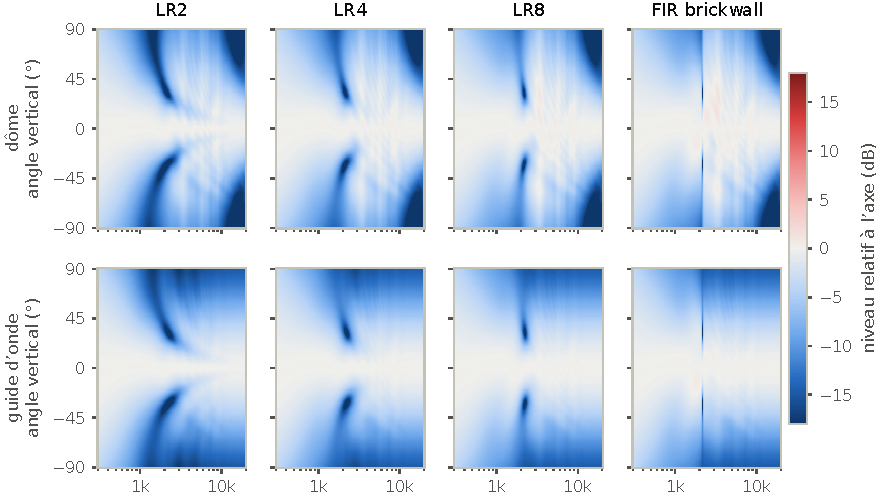
\includegraphics[width=\textwidth]{polar_maps}
\caption{Directivité de la deux voies dans le plan vertical, relative à la réponse dans l'axe, avec les
quatre filtres~: dôme nu (en haut), dôme en guide d'onde (en bas).}
\label{fig:polar}
\end{figure}

% =============================================================================================
\section{Les pièces}
\label{sec:rooms}

\subsection{Modèle}

Les pièces sont des parallélépipèdes rectangles. Dans le repère de la pièce, $x$ la traverse, $y$ va du
mur derrière l'auditeur au mur derrière les enceintes, $z$ monte. Le son qui atteint l'auditeur se
décompose en trois parties, toutes en énergie.

\paragraph{Sources images,} jusqu'au troisième ordre \cite{allen1979}. Sur chaque axe, avec des parois
en 0 et en $L$, l'image de la source $s$ est $u = 2nL + (1 - 2q)s$ ($n$ entier, $q \in \{0, 1\}$)~; elle a
rebondi $|n - q|$ fois sur la paroi en 0 et $|n|$ fois sur celle en $L$. L'enceinte émet ce trajet dans
la direction $\vect P(\vect r - \vect u)/|\vect r - \vect u|$, où $\vect P$ retourne les axes qui comptent
un nombre impair de rebonds ($q = 1$) et $\vect r$ désigne la tête de l'auditeur. Son poids vaut
\begin{equation}
W = \frac{e^{-m |\vect r - \vect u|}}{|\vect r - \vect u|^2}\,\prod_{\text{rebonds}} (1 - \alpha)(1 - s),
\end{equation}
où $\alpha$ est le coefficient d'absorption, $s$ le coefficient de diffusion (la part de l'énergie
réfléchie renvoyée dans toutes les directions plutôt que dans la direction spéculaire) et $m$
l'atténuation en énergie par mètre de l'air \cite{iso9613}, et du mobilier au-delà du premier ordre.

\paragraph{Champ diffus.} Un rayon lancé depuis l'enceinte dans la direction $\Omega$ est suivi dans la
boîte. À chacun de ses trois premiers rebonds, la part diffusée $(1 - \alpha)s$ de l'énergie qu'il
transporte rejoint un champ diffus~; après le troisième, tout ce qui reste le rejoint. On définit ainsi
$g(\Omega) \in [0, 1]$, la part de l'énergie émise dans la direction $\Omega$ qui alimente le champ diffus.
En régime établi, ce champ donne partout
\begin{equation}
p^2_{\mathrm{diff}} = \frac{4}{A}\oint g(\Omega)\,P(\Omega)\dd\Omega, \qquad
A = -S\ln(1 - \bar\alpha) + 4 m V,
\end{equation}
avec l'aire d'absorption d'Eyring de toute la pièce, air et mobilier compris \cite{kuttruff2016}. Avec
$g = 1 - \alpha$ partout, on retrouve le terme de salle $4/R$ de Hopkins et Stryker \cite{hopkins1948}.
L'intégrale porte sur les 3000 directions d'un réseau de Fibonacci.

\paragraph{Son direct,} l'image d'ordre 0.

Des zones absorbantes (un tapis, des panneaux, un nuage au plafond) remplacent les coefficients d'une
paroi là où un rayon ou une réflexion du premier ordre les atteint~; les images d'ordre supérieur et le
champ diffus utilisent la moyenne de chaque paroi pondérée par les surfaces. Le mobilier est une aire
d'absorption équivalente $A_f$ répartie dans le volume, soit une atténuation $m_f = A_f / 4V$ par mètre
appliquée aux images d'ordre 2 et plus, aux rayons et au champ diffus~; le son direct et les premières
réflexions sont supposés dégagés.

L'énergie reçue par l'auditeur s'écrit alors
\begin{equation}
E(f) = \sum_{\text{images}} W_k(f)\,P(\Omega_k, f) + \sum_{\text{réseau}} \frac{4}{A}\,\frac{4\pi}{N}\,g(\Omega_l, f)\,P(\Omega_l, f),
\end{equation}
un jeu de poids sur les directions, comme les courbes de la norme. Nous la donnons relativement à une
source omnidirectionnelle placée au même endroit ($P \equiv 1$), ce qui retire la coloration propre de
la pièce (son absorption qui croît avec la fréquence)~: $E(f) / E_{\mathrm{omni}}(f)$ décrit la façon dont
la pièce pondère les directions de l'enceinte, la grandeur qu'estime la PIR. Une enceinte qui rayonne
la même chose partout obtient 0\,dB dans toutes les pièces. Deux versions~: le \emph{régime établi},
tous les trajets, et le \emph{son précoce}, le son direct et les six premières réflexions, ce que
représentent la LW et l'ER.

\subsection{Vérifications}

Dans une pièce d'absorption uniforme, le modèle coïncide à 1\,\% près avec Hopkins--Stryker quand toutes
les réflexions sont diffusantes ($s = 1$). Quand aucune ne l'est ($s = 0$), son énergie totale reste à 3
à 7\,\% (0,15 à 0,3\,dB) de celle d'une méthode des images complète sommée jusqu'au 26\ieme{} ou au
40\ieme{} ordre (25\,000 et 88\,000 images), pour $\bar\alpha = 0,25$ et 0,1. Les coefficients de
diffusion des pièces (0,05 à 0,5) se situent entre ces deux cas.

\subsection{L'ensemble de pièces}

Chaque configuration comprend l'enceinte gauche d'une paire stéréo et un auditeur sur l'axe médian de
la pièce (l'enceinte droite est son image en miroir). Les 300 configurations aléatoires
(tableau~\ref{tab:ensemble}) tirent une largeur de 3,4 à 5,2\,m, une longueur de 4,5 à 7,5\,m et une
hauteur de 2,4 à 2,8\,m~; des enceintes contre le petit mur, leur baffle à 0,4--1,2\,m de celui-ci,
écartées de 1,8 à 2,8\,m et à 0,45\,m au moins des murs latéraux, l'axe de référence à 0,85--1,15\,m du
sol~; un auditeur à 2,0--3,8\,m de la ligne des baffles et à 0,5\,m au moins devant le mur derrière lui,
les oreilles à 1,0--1,25\,m~; des enceintes pincées vers l'auditeur (la moitié des cas), parallèles aux
murs latéraux (un quart) ou à mi-chemin (un quart). Les murs sont en plâtre peint sur maçonnerie ou en
plaques de plâtre sur ossature, l'un d'eux avec une fenêtre (2--6\,m$^2$) et des rideaux (0--4\,m$^2$)~;
le plafond en plâtre ou en plaques~; le sol en parquet ou en carrelage (60\,\% des cas, dont la moitié
avec un tapis de 2--3\,m sur 2,5--3,5\,m devant les enceintes) ou en moquette~; le mobilier absorbe 6 à
16\,m$^2$ à 1\,kHz, moitié moins à 125\,Hz. Un quart des pièces (\ntreated) est traité~: panneaux de laine
minérale de 50\,mm, de $1,2 \times 1,2$\,m, aux points de première réflexion des murs latéraux, et un
tapis~; le plafond reste nu. Les coefficients d'absorption et de diffusion sont des valeurs typiques
des manuels~; les temps de réverbération (\nrtMedian\,s en médiane à 1\,kHz, de \nrtLo\ à \nrtHi\,s pour
80\,\% des pièces) tombent dans la plage mesurée dans les logements meublés \cite{diaz2005}. Les 150
premières pièces servent à ajuster les poids mis à jour, les 150 autres à les tester.

\begin{table}[t]
\centering
\caption{Les 300 configurations aléatoires~: 10\ieme{} centile, médiane, 90\ieme{} centile.}
\label{tab:ensemble}
\begin{tabular}{lrrr}
\toprule
& 10\,\% & médiane & 90\,\% \\
\midrule
\rows{ensemble}
\bottomrule
\end{tabular}
\end{table}

\begin{figure}[t]
\centering
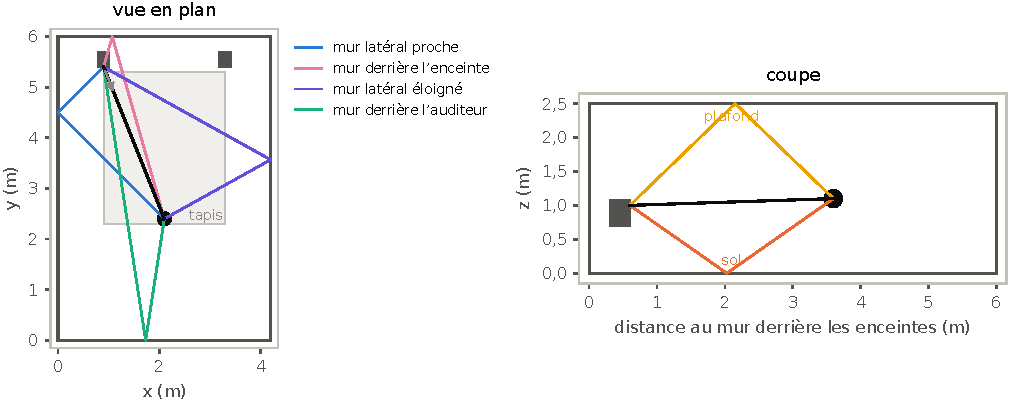
\includegraphics[width=\textwidth]{setup}
\caption{L'une des pièces ($4,2 \times 6,0 \times 2,5$\,m, parquet et tapis)~: l'enceinte gauche,
l'auditeur, le son direct (en noir) et les six premières réflexions.}
\label{fig:setup}
\end{figure}

% =============================================================================================
\section{La norme face aux pièces}
\label{sec:standard}

\subsection{Où va l'énergie}

Pour une source omnidirectionnelle, le son direct apporte \ndirectShare\,\% de l'énergie en régime
établi à 1\,kHz (médiane), les six premières réflexions \nfirstShare\,\% à elles toutes, les trajets plus
tardifs \nlateShare\,\% (tableau~\ref{tab:shares}, figure~\ref{fig:shares}). La PIR donne 12\,\% à la
fenêtre d'écoute, 44\,\% aux premières réflexions et 44\,\% à la puissance, soit à peu près le double de la
part du son direct et quatre fois celle des premières réflexions.

Parmi les premières réflexions, le sol et le plafond apportent \nvertShare\,\% de l'énergie (de \nvertLo\
à \nvertHi\,\%), les murs latéraux \nsideShare\,\%. C'est la part que leur donnent les premières réflexions
de la norme, deux rebonds sur cinq. Dans les pièces traitées, le sol et le plafond montent à
\nvertTreated\,\% (\nvertUntreated\,\% dans les autres). Le plafond l'emporte sur le sol~: tapis et
moquettes absorbent le rebond sur le sol, et le mobilier posé au sol le diffuse.

\begin{table}[t]
\centering
\caption{Part de l'énergie reçue par l'auditeur (\%), source omnidirectionnelle~: médiane et plage de
10 à 90\,\% sur les 300 pièces.}
\label{tab:shares}
\begin{tabular}{lrrrr}
\toprule
& \multicolumn{2}{c}{1\,kHz} & \multicolumn{2}{c}{4\,kHz} \\
& médiane & plage & médiane & plage \\
\midrule
\rows{shares}
\bottomrule
\end{tabular}
\end{table}

\begin{figure}[t]
\centering
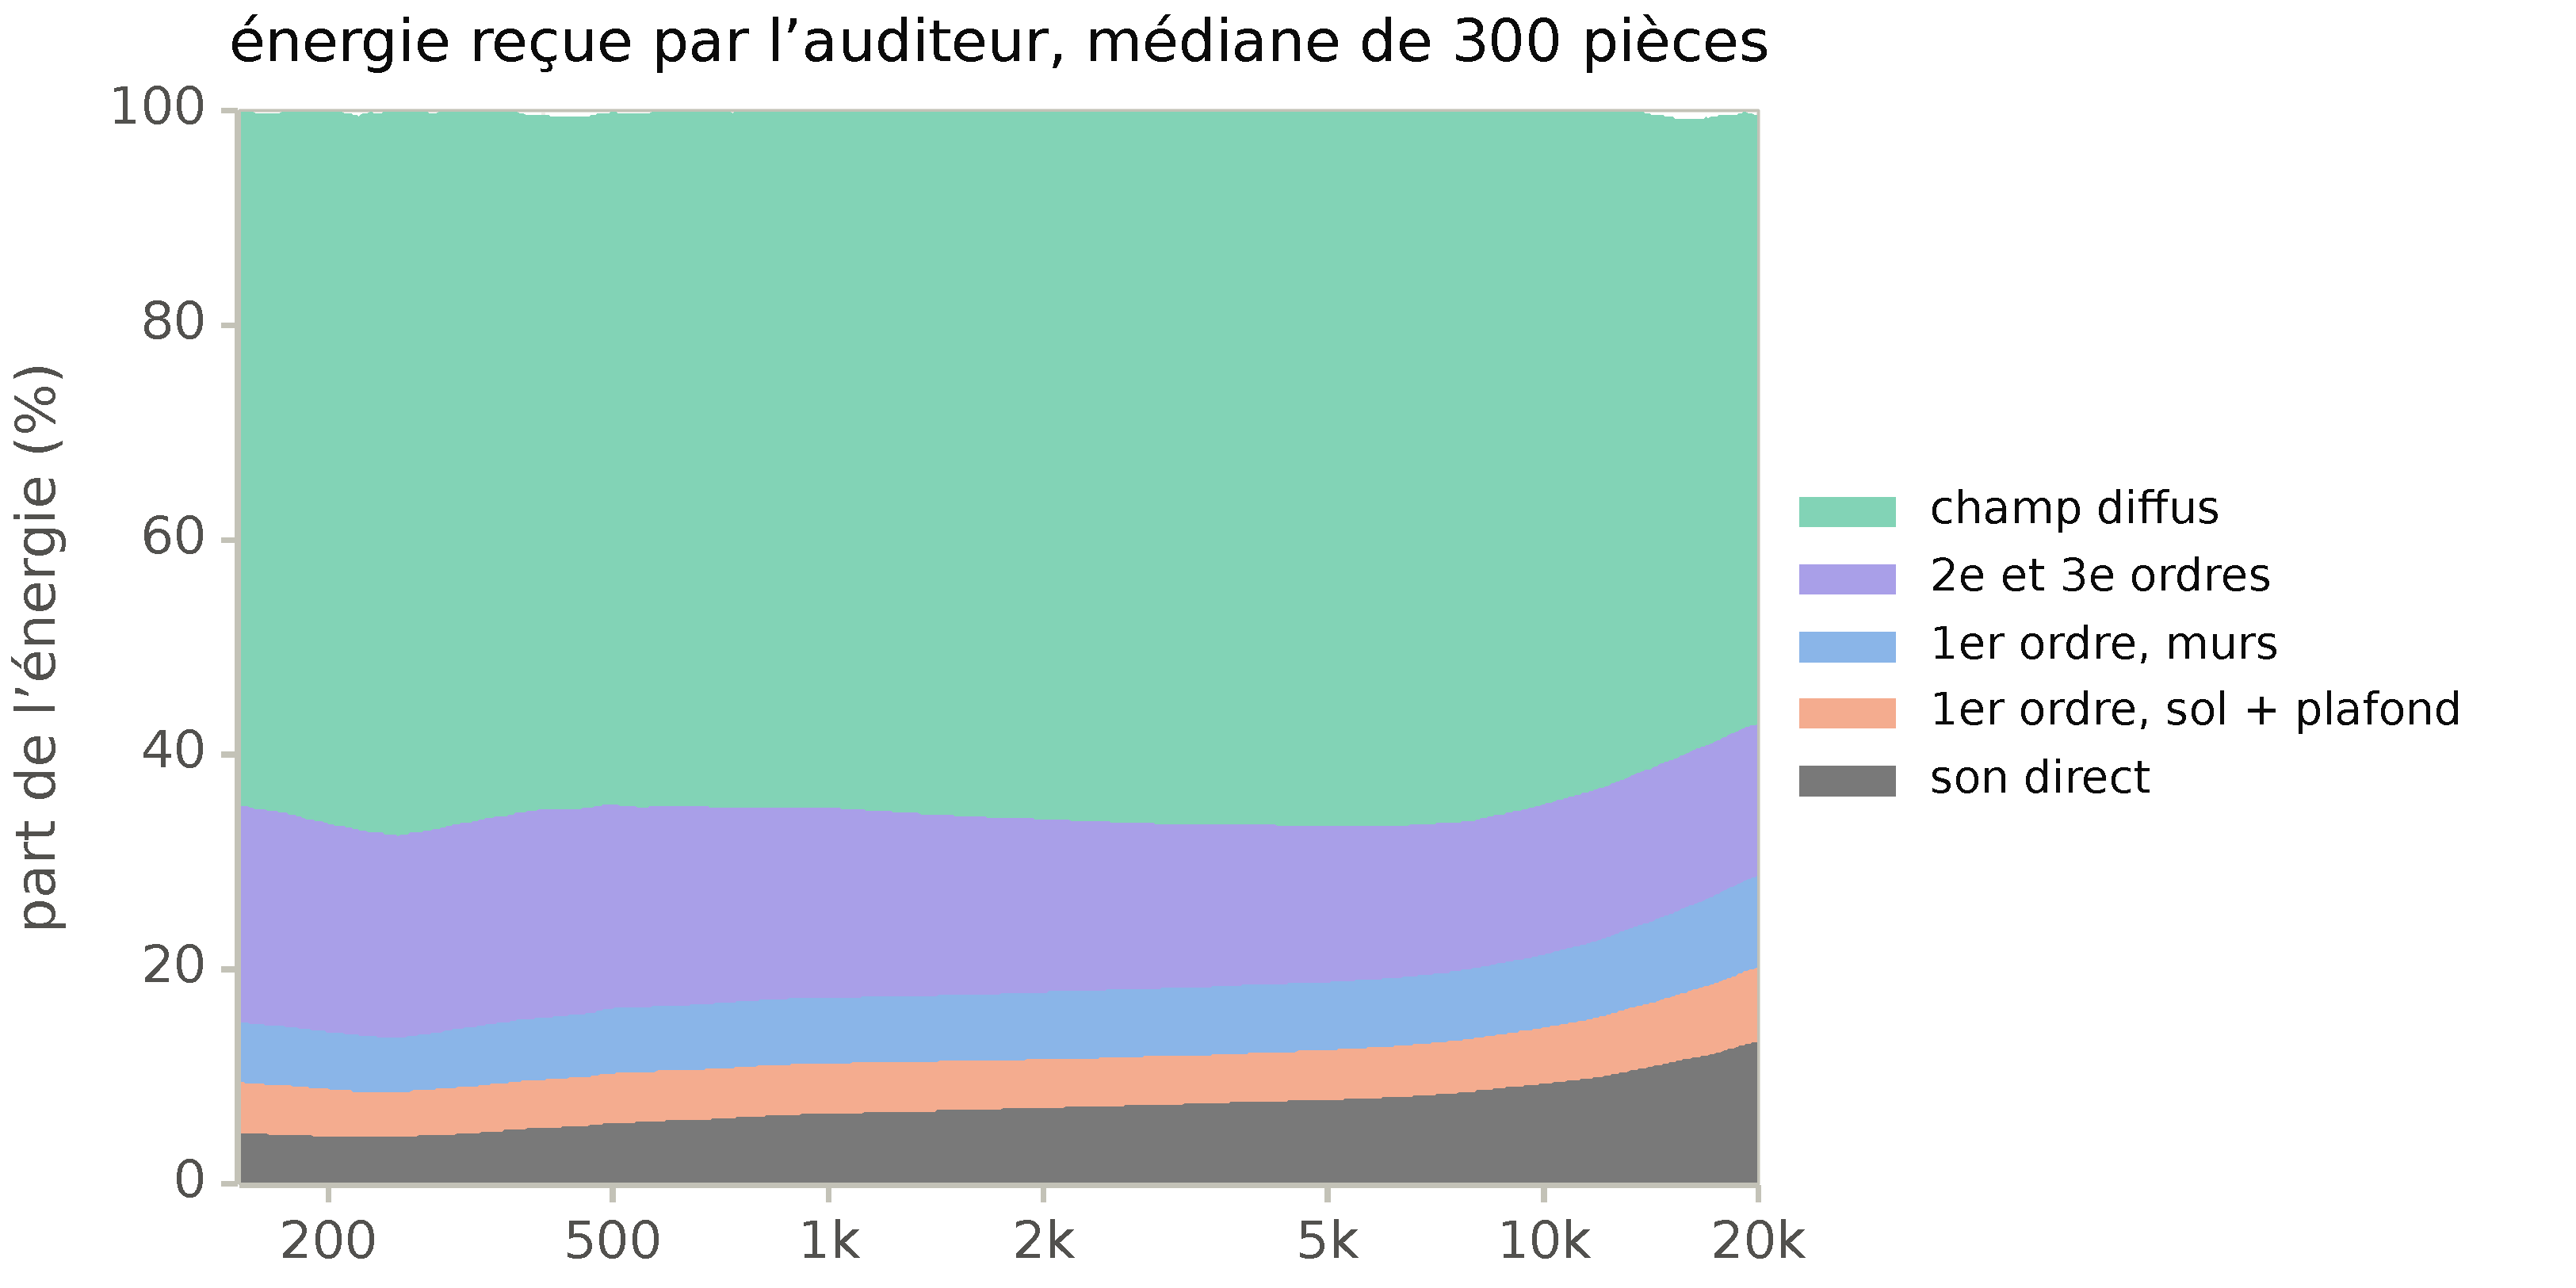
\includegraphics[width=0.75\textwidth]{shares}
\caption{Part de l'énergie reçue par l'auditeur selon le type de trajet, source omnidirectionnelle,
médiane des 300 pièces.}
\label{fig:shares}
\end{figure}

\subsection{Dans quelles directions}

Les premières réflexions quittent l'enceinte là où la norme les cherche (tableau~\ref{tab:directions},
figures~\ref{fig:kernels} et~\ref{fig:angles}). Le rebond sur le sol part à $\nangleFloor^\circ$
(médiane), celui sur le plafond à $\nangleCeiling^\circ$~; les angles de la norme pour le sol et le plafond
les encadrent, ses $-20^\circ$ et $60^\circ$ correspondant à des auditeurs plus éloignés ou plus proches.
Ces deux rebonds arrivent les premiers, \ndelayFloor\ et \ndelayCeiling\,ms après le son direct, avec
celui du mur latéral proche (\ndelayLeft\,ms)~: dans des pièces plus larges que hautes, le sol et le
plafond sont les parois les plus proches. Les rebonds sur les murs latéraux tombent dans les $\pm40$ à
$\pm80^\circ$ de la norme, celui sur le mur derrière l'auditeur (le \og mur avant\fg{} de la norme) dans ses
$\pm30^\circ$. Le mur derrière les enceintes (son \og mur arrière\fg{}) est atteint entre $137$ et
$166^\circ$, là où la norme regarde à $\pm90^\circ$ et $180^\circ$.

\begin{table}[t]
\centering
\caption{Directions dans lesquelles les premières réflexions quittent l'enceinte (degrés, médiane et
plage de 10 à 90\,\% sur les 300 pièces), angles de la norme (V orbite verticale, H orbite horizontale)
et retard des réflexions sur le son direct (médiane).}
\label{tab:directions}
\small
\begin{tabular}{llrrlr}
\toprule
réflexion & angle & médiane & plage & CTA-2034 & retard (ms) \\
\midrule
\rows{directions}
\bottomrule
\end{tabular}
\end{table}

\begin{figure}[t]
\centering
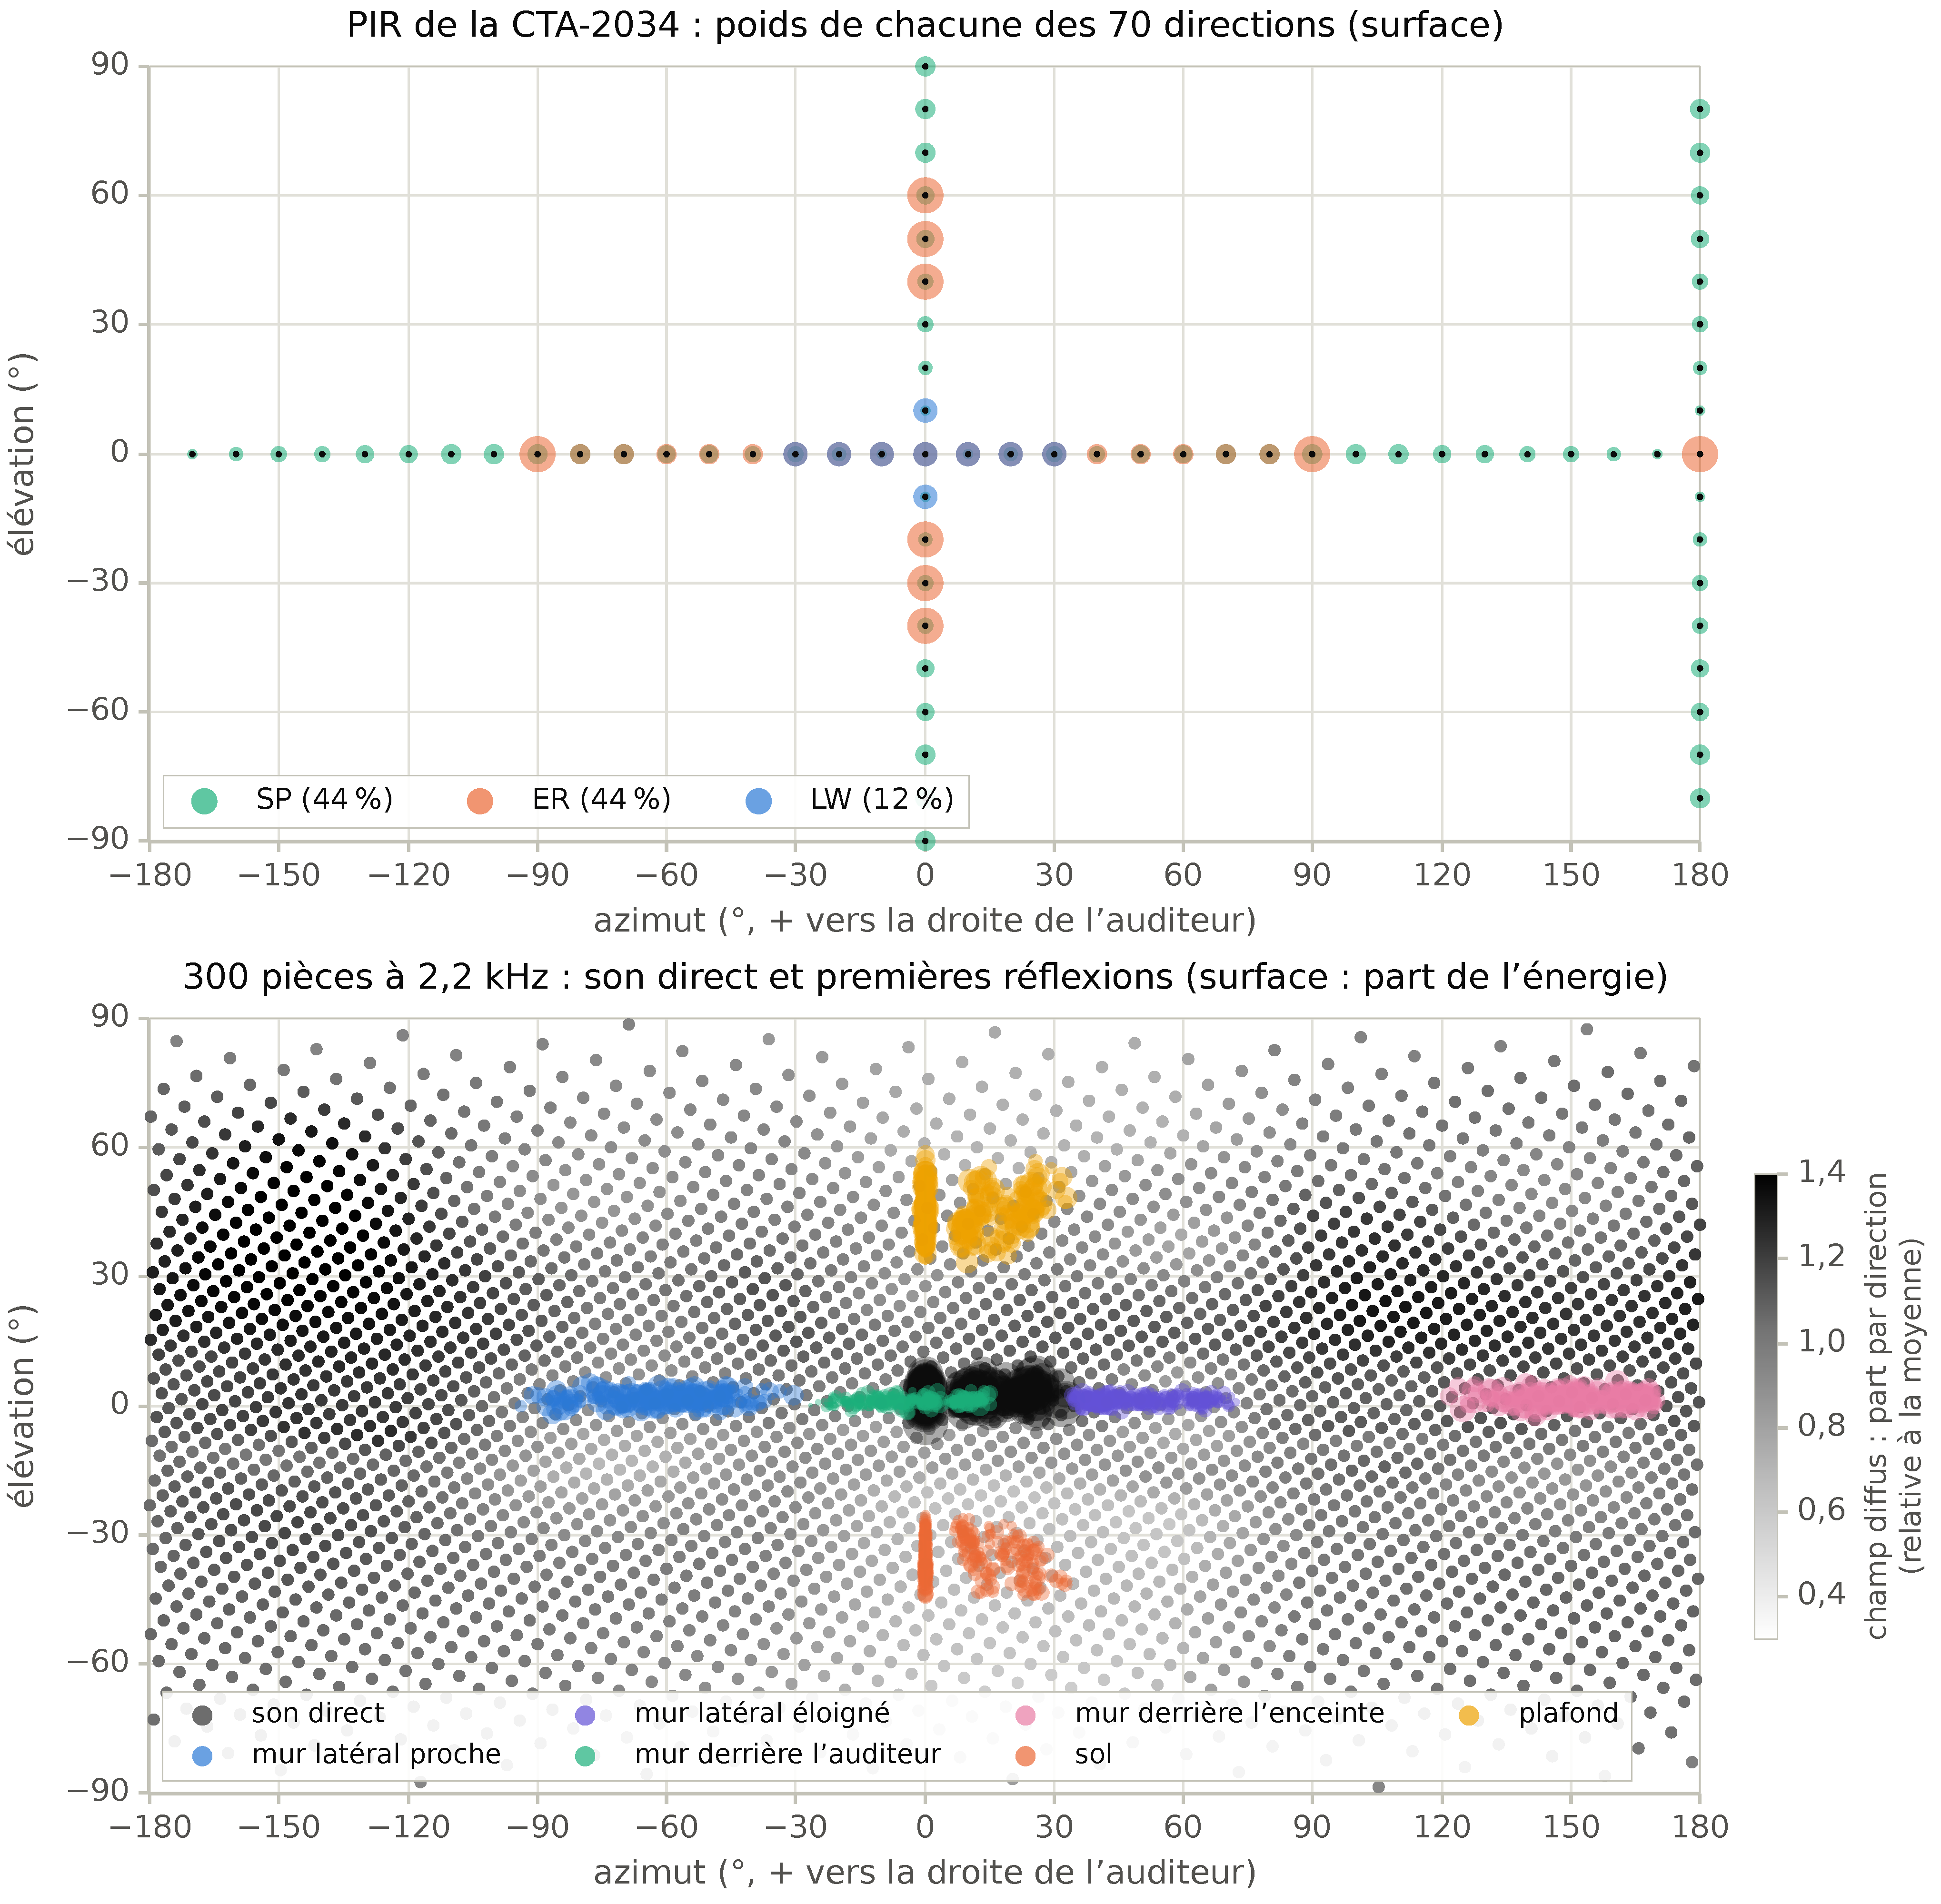
\includegraphics[width=\textwidth]{kernel_maps}
\caption{En haut~: le poids que la PIR donne à chacune des 70 directions (surface des cercles), réparti
entre ses parts LW, ER et SP~; au-delà de $90^\circ$, l'orbite verticale est tracée à l'azimut $180^\circ$.
En bas~: les 300 pièces à 2,2\,kHz, le son direct et les premières réflexions (surface~: part de
l'énergie reçue), sur fond de la part du champ diffus par direction $g$, relative à sa moyenne (en
gris).}
\label{fig:kernels}
\end{figure}

\begin{figure}[t]
\centering
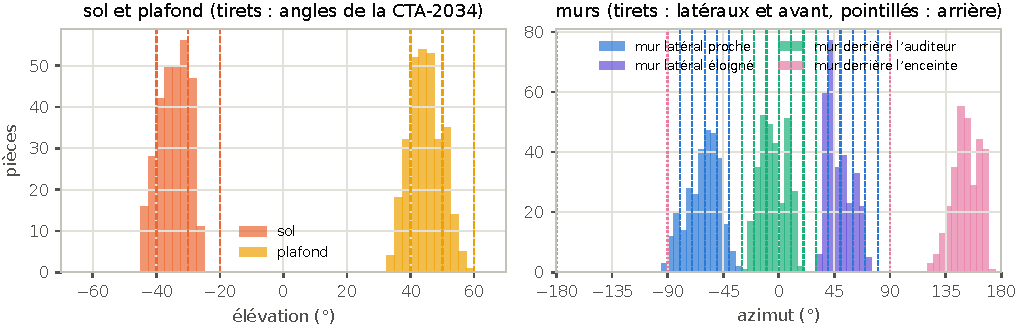
\includegraphics[width=\textwidth]{reflection_angles}
\caption{Directions des premières réflexions dans les 300 pièces, et angles de la norme.}
\label{fig:angles}
\end{figure}

Le champ diffus ne puise pas non plus également dans toutes les directions (figure~\ref{fig:kernels}, en
bas)~: ce que l'enceinte envoie vers un sol absorbant ou un tapis l'alimente moins que ce qu'elle envoie
vers l'arrière ou vers le haut. Les écarts atteignent environ $\pm30$\,\%, bien moins que le contraste
que la norme établit entre les directions de l'ER et les autres.

\subsection{Prédire la réponse dans la pièce}
\label{sec:prediction}

Avec des poids de somme unité ajustés sur les 150 pièces d'apprentissage, les seize variantes d'enceinte
ensemble, la réponse en régime établi est le mieux prédite par
\begin{equation}
\nwLw\,\mathrm{LW} + \nwEr\,\mathrm{ER} + \nwSp\,\mathrm{SP}_{\text{sphère}},
\end{equation}
avec la puissance intégrée sur la sphère, ou par $\nwLwTwo\,\mathrm{LW} + \nwErTwo\,\mathrm{ER} +
\nwSpTwo\,\mathrm{SP}$ avec celle des deux orbites (tableau~\ref{tab:errors}, figure~\ref{fig:errors}).
Ajusté sur des sous-ensembles (pièces traitées, temps de réverbération inférieurs à 0,33\,s ou
supérieurs à 0,5\,s, auditeurs à moins de 2,6\,m ou à plus de 3,2\,m), le poids de la LW reste entre 0,07
et 0,16 et celui de l'ER entre $-0,05$ et 0,04. Ajustés sur le seul dôme nu, les poids prédisent le
guide d'onde aussi bien que son propre ajustement. Les premières réflexions n'apportent rien à la
prédiction~: leurs directions sont celles d'une faible part de l'énergie, que la LW et la SP décrivent
déjà. Sur les pièces de test, ces poids sont aussi proches de chaque pièce que la moyenne des pièces
d'apprentissage, le plancher que fixe la dispersion entre pièces. La PIR s'en écarte de 1,7 à
2,1\,dB RMS, surtout par un biais~: elle se tient \npirBiasLow\,dB au-dessus des pièces à 300\,Hz et
jusqu'à \npirBiasMax\,dB au-dessus au raccordement, parce qu'elle s'appuie sur la fenêtre d'écoute, là
où une enceinte directive vers l'avant est la plus forte (figure~\ref{fig:spin}).

Pour le son précoce seul, les pièces pondèrent environ $\nwLwEarly\,\mathrm{LW} + \nwErEarly\,\mathrm{ER}
+ \nwSpEarly\,\mathrm{SP}$~: le son direct en apporte \nearlyDirect\,\%, quand la partie précoce de la PIR
($0,12\,\mathrm{LW} + 0,44\,\mathrm{ER}$, normalisée) donne 21\,\% à la fenêtre d'écoute.

\begin{table}[t]
\centering
\caption{Prédiction de la réponse en régime établi des 150 pièces de test, de 300\,Hz à 16\,kHz~:
erreur RMS médiane sur les pièces et plus grande erreur moyenne (biais) sur la fréquence, plage sur les
seize variantes (dB).}
\label{tab:errors}
\small
\begin{tabular}{lrr}
\toprule
prédiction & erreur RMS & plus grand biais \\
\midrule
\rows{errors}
\bottomrule
\end{tabular}
\end{table}

\begin{figure}[t]
\centering
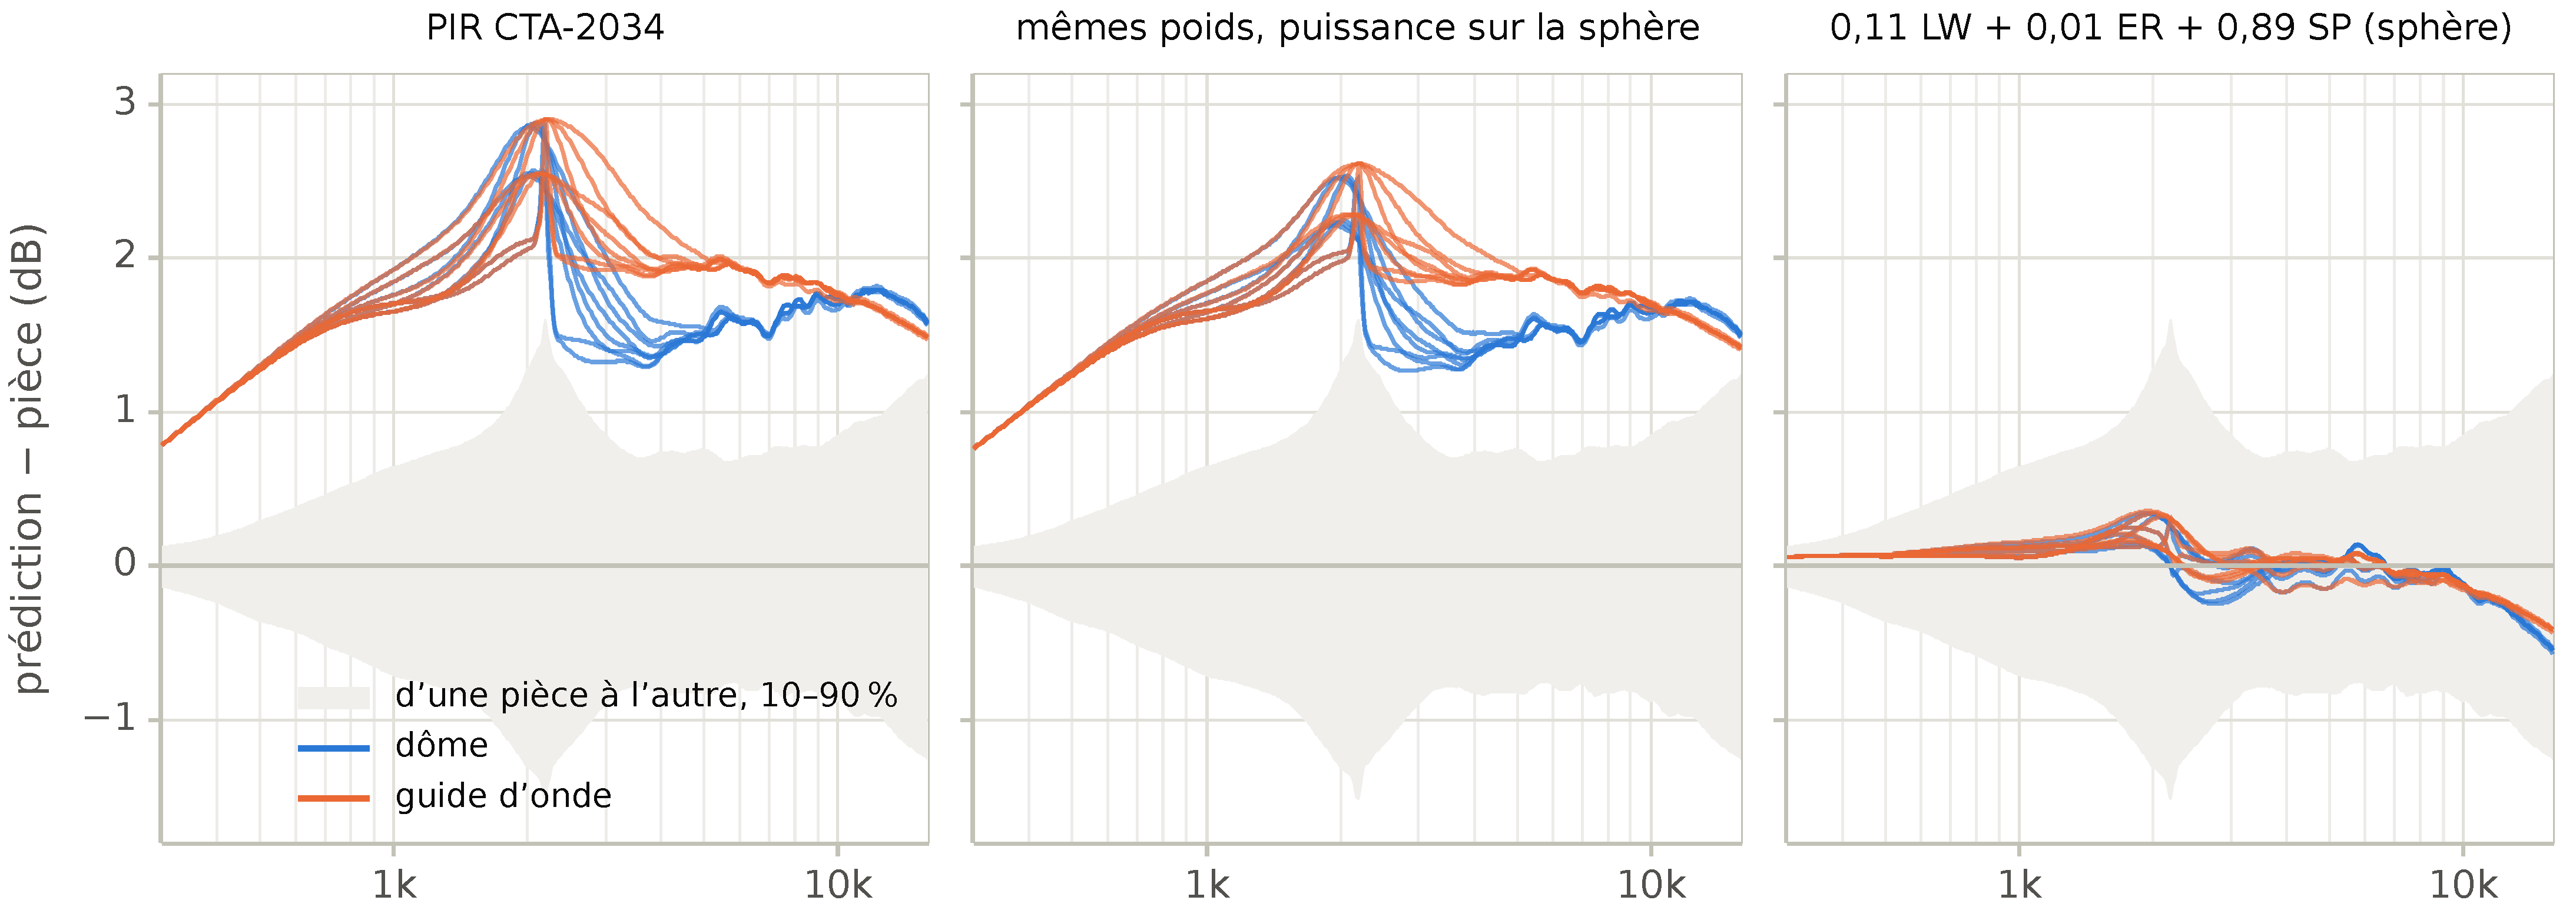
\includegraphics[width=\textwidth]{errors}
\caption{Erreur moyenne de trois prédictions sur les 150 pièces de test, pour chaque variante (traits
fins), et dispersion propre des pièces autour de leur moyenne (en gris).}
\label{fig:errors}
\end{figure}

\begin{figure}[t]
\centering
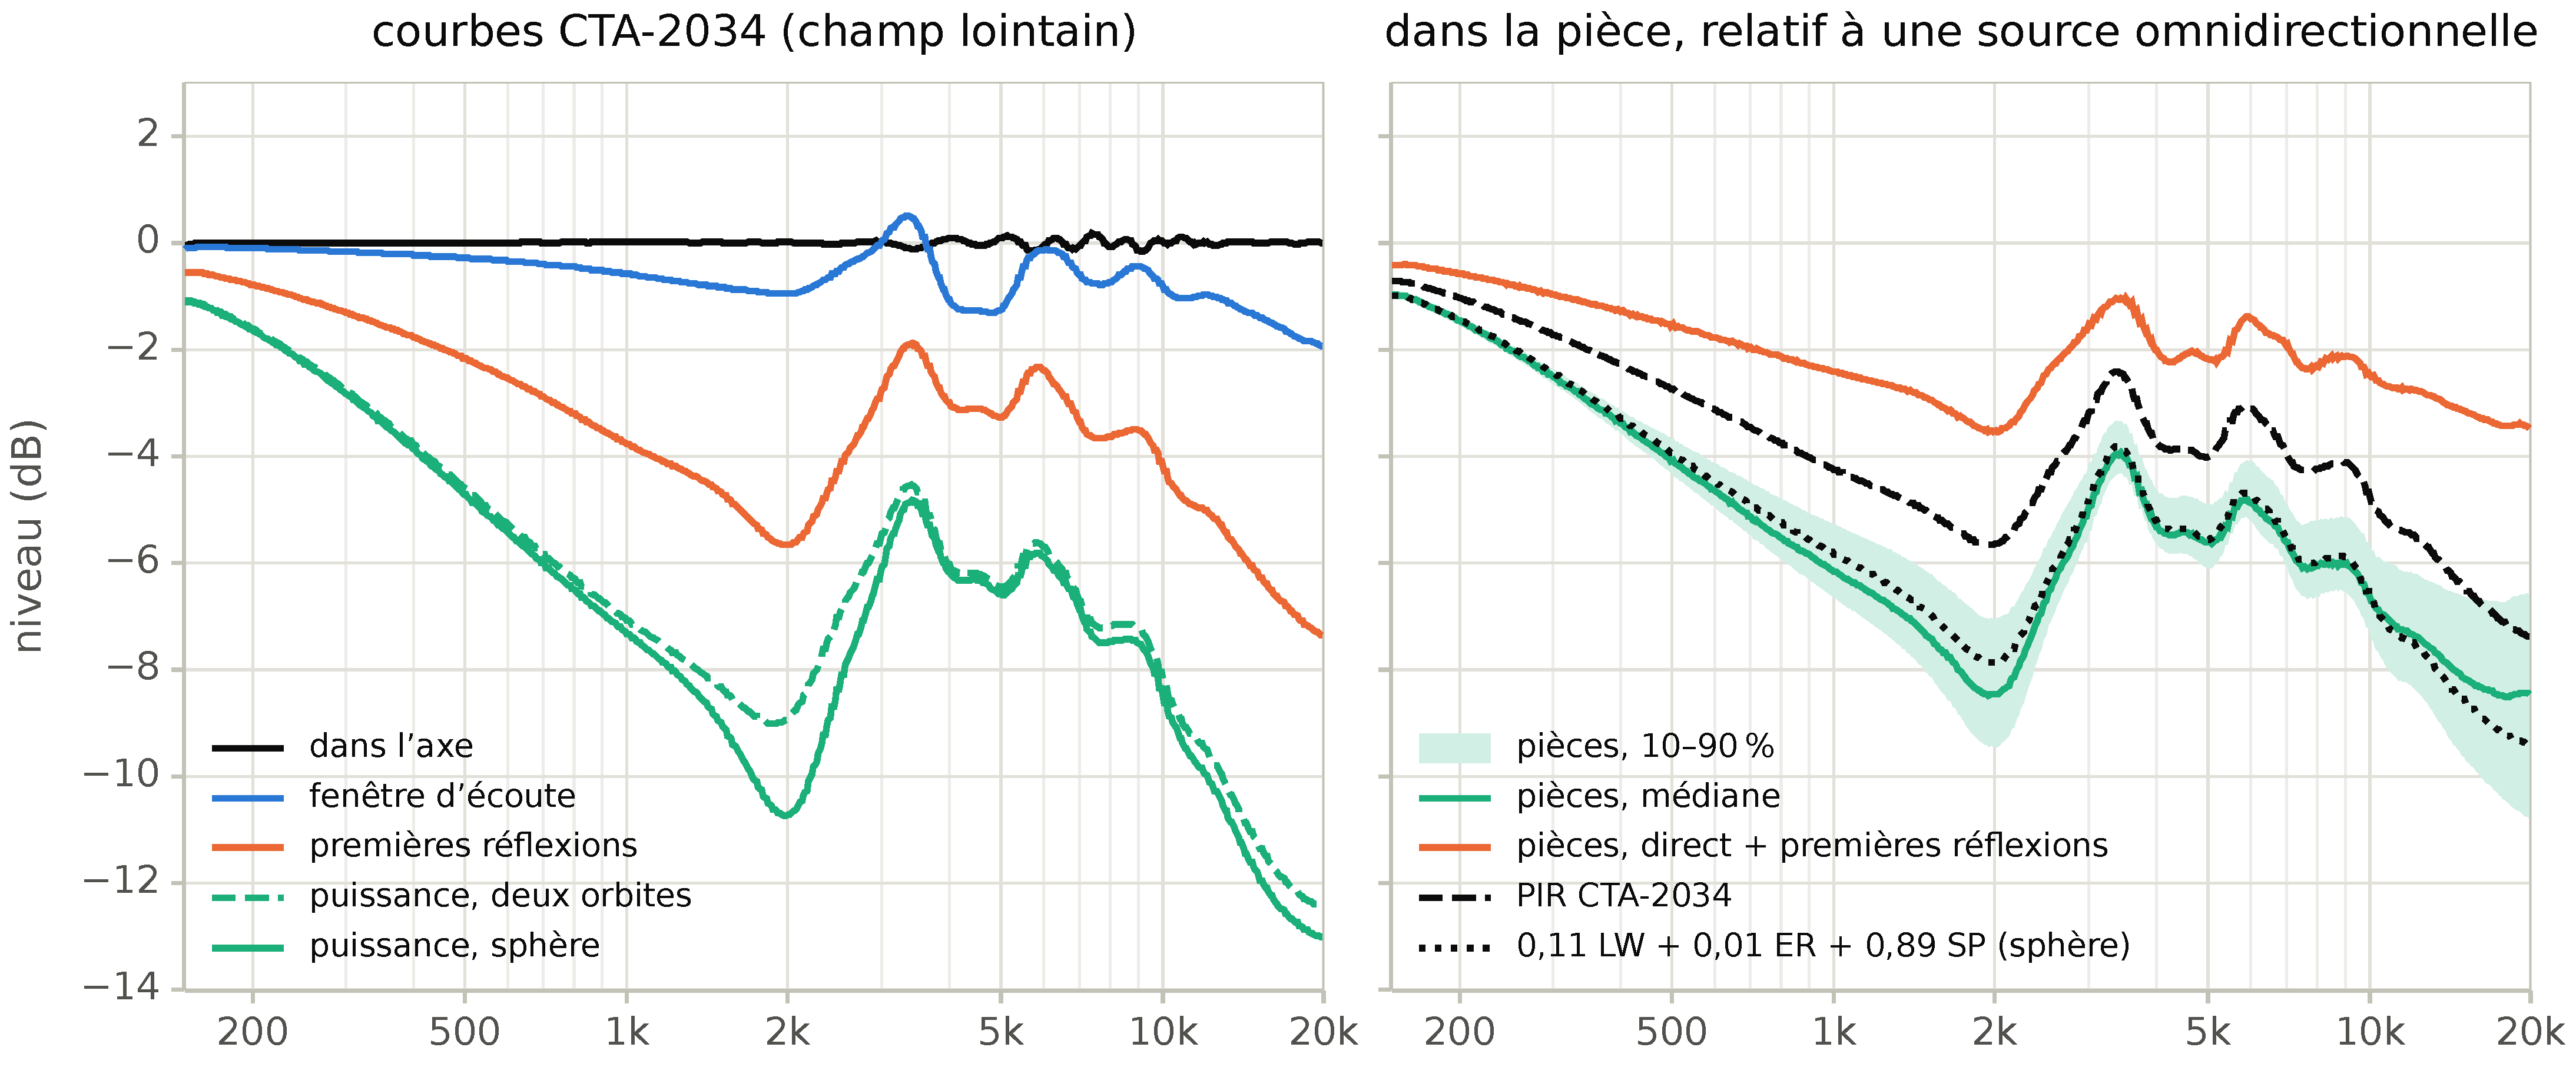
\includegraphics[width=\textwidth]{spin_dome}
\caption{La deux voies debout, dôme nu, LR4. À gauche~: ses courbes CTA-2034, la puissance sur deux
orbites et sur la sphère. À droite~: dans les pièces, relativement à une source omnidirectionnelle, en
régime établi (médiane et plage de 10 à 90\,\%) et pour le son précoce (médiane), avec la PIR et les
poids ajustés.}
\label{fig:spin}
\end{figure}

\subsection{La puissance sur deux orbites}
\label{sec:sp}

Autour du raccordement, les deux haut-parleurs jouent ensemble, et les lobes entre eux coûtent de la
puissance. L'orbite horizontale de l'enceinte debout ne voit aucune interférence, puisque les deux
haut-parleurs sont à la même distance d'elle~; l'orbite verticale la voit. Les deux orbites reçoivent le
même poids, alors que seule une mince bande de la sphère autour du plan horizontal est épargnée. À
2\,kHz, la puissance sur deux orbites est trop haute de \nspBiasLrFour\,dB avec le LR4 (\nspBiasLrTwo\
avec le LR2, \nspBiasLrEight\ avec le LR8~; figure~\ref{fig:sporbits})~: des 2,6\,dB dont la puissance du
LR4 tombe sous celle du brickwall à cette fréquence, les deux orbites en montrent 1,2. Il en va de même
pour l'enceinte couchée, les orbites échangeant leurs rôles. Au-dessus du raccordement, les deux
orbites surestiment le dôme directif de 0,2 à 0,6\,dB, effet des carrés sphériques (section~\ref{sec:cta}).

\begin{figure}[t]
\centering
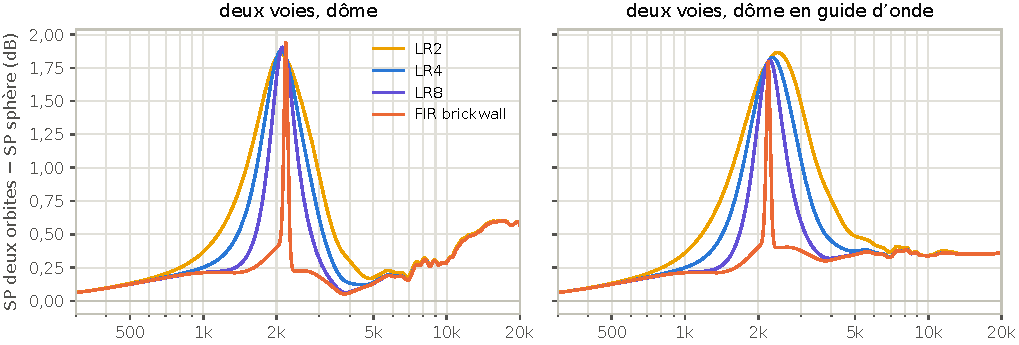
\includegraphics[width=\textwidth]{sp_orbits}
\caption{Puissance sur les deux orbites moins puissance sur la sphère, deux voies debout.}
\label{fig:sporbits}
\end{figure}

\subsection{Debout ou couchée}

Couchée sur le flanc, l'enceinte forme ses lobes à l'horizontale au lieu de la verticale. La fenêtre
d'écoute voit la différence (figure~\ref{fig:rotation})~: un creux d'environ 1\,dB à 2\,kHz debout, de 2,3
à 2,6\,dB couchée~; la PIR bouge à peine. Le régime établi des pièces ne bouge pas davantage~: il est
surtout fait de puissance, qui ne dépend pas de l'orientation. Le son précoce, lui, change, mais pas
dans sa médiane. Debout, aucune pièce ne laisse l'auditeur plus de 1,1\,dB sous la médiane au
raccordement~; couchée, un quart des pièces le laissent plus de 3\,dB en dessous, une sur dix 5,7\,dB.
Ce sont des configurations où les enceintes ne sont pas pincées vers l'auditeur, qui se trouve alors à
23--$33^\circ$ de l'axe, près du premier zéro des lobes ($34^\circ$ à 2,2\,kHz). Un auditeur assis reçoit le
son direct à moins de $5^\circ$ de l'axe verticalement (90\,\% des pièces) et jusqu'à $24^\circ$
horizontalement~; les $\pm30^\circ$ horizontaux et $\pm10^\circ$ verticaux de la fenêtre d'écoute suivent
cette asymétrie. Les lobes verticaux atteignent l'auditeur par les rebonds sur le sol et le plafond et
par le champ réverbéré, que l'ER et la SP portent, en moyenne (section~\ref{sec:crossovers}).

\begin{figure}[t]
\centering
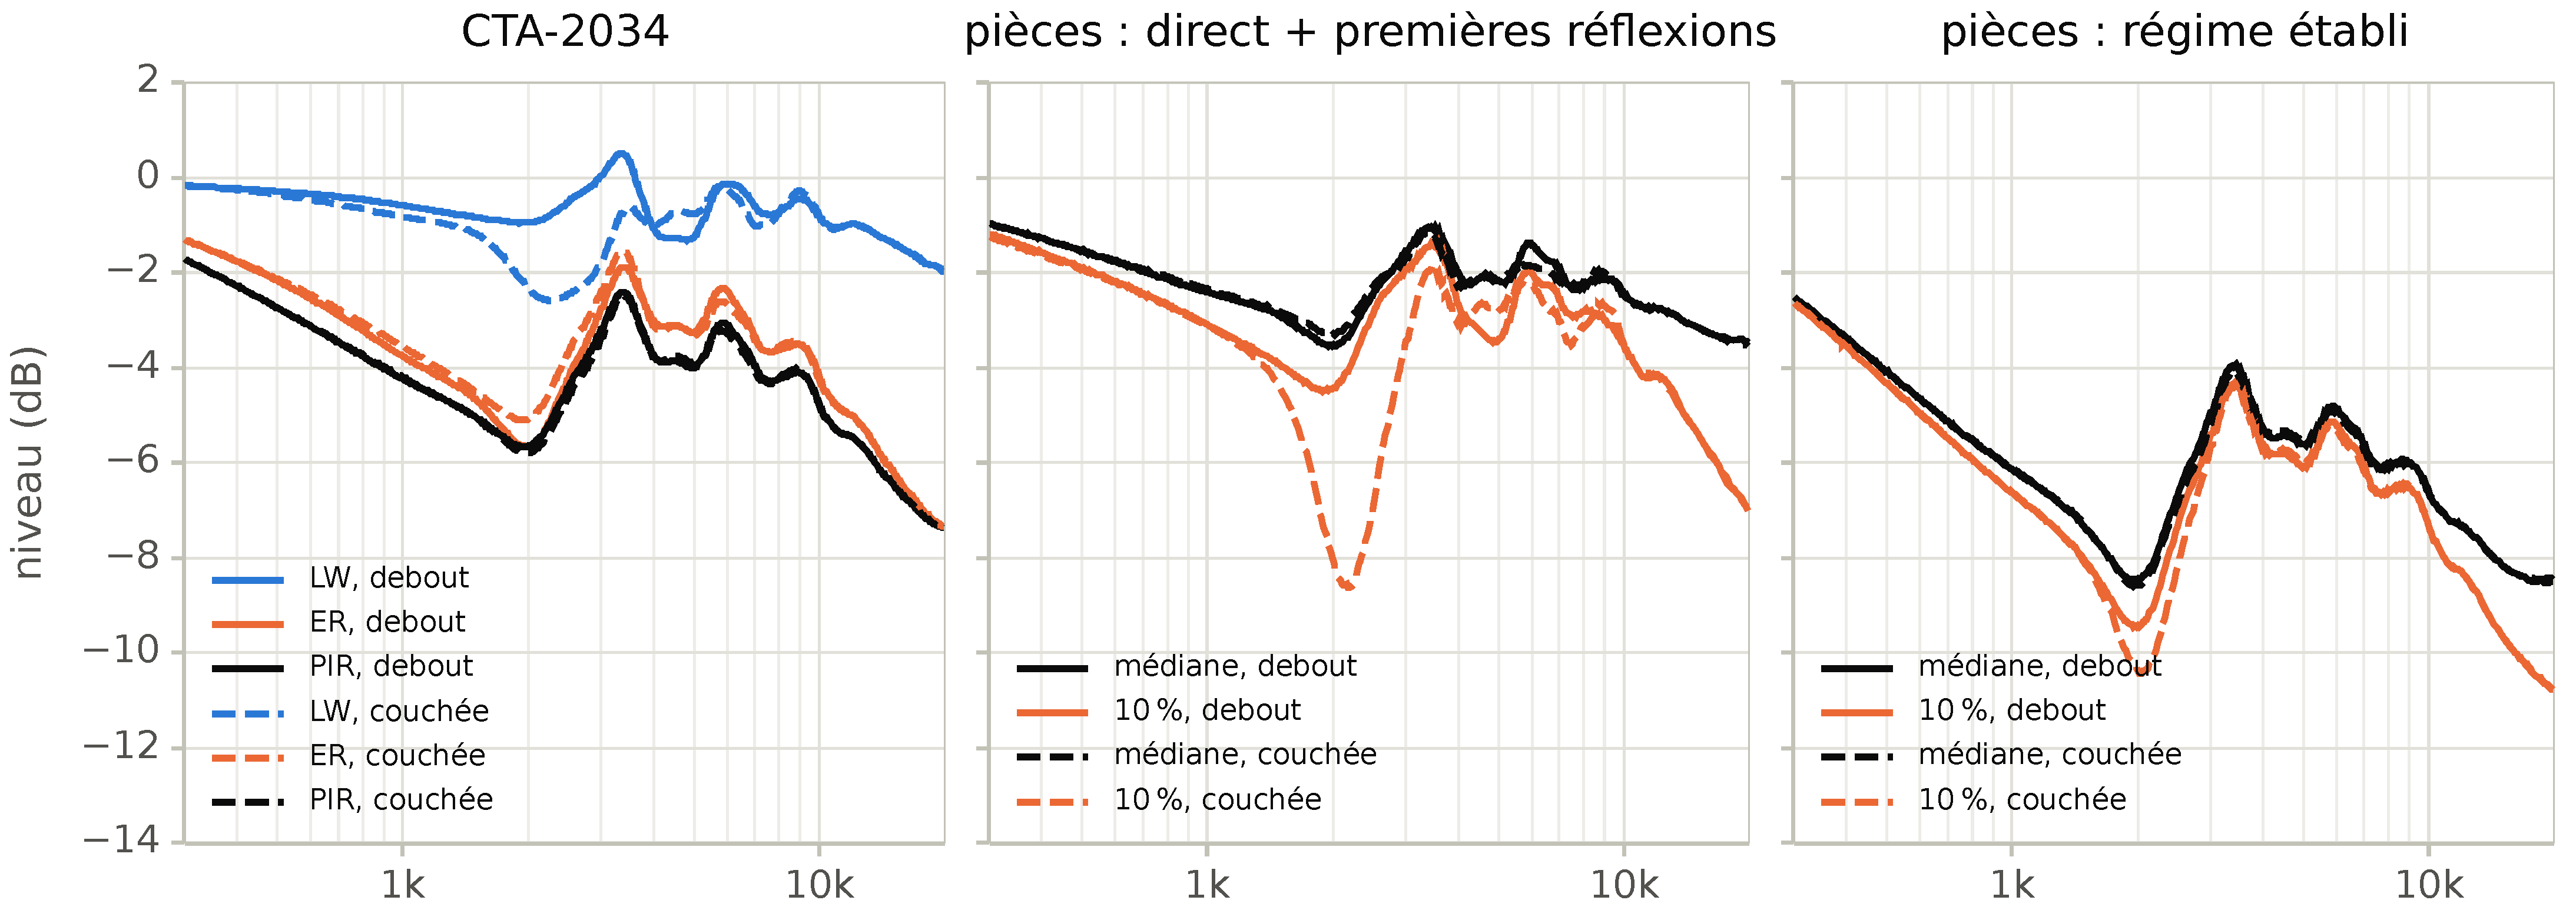
\includegraphics[width=\textwidth]{rotation}
\caption{La deux voies en LR4, debout et couchée. À gauche~: ses LW, ER et PIR. Au centre et à droite~: les
pièces, son précoce et régime établi, médiane et 10\ieme{} centile.}
\label{fig:rotation}
\end{figure}

% =============================================================================================
\section{Linkwitz-Riley face au FIR brickwall}
\label{sec:crossovers}

\subsection{Moyennes et trajets}

Les défauts d'un filtre se situent à moins d'une octave environ de sa fréquence, et, dans chaque
direction, à une fréquence qui lui est propre~: deux haut-parleurs distants de $d$ s'annulent là où
$d \sin\theta$ vaut une demi-longueur d'onde, à $34^\circ$ pour 2,2\,kHz et 140\,mm, sous des angles plus
ouverts aux fréquences plus basses. Sommer des directions en puissance, comme le font la courbe dans la
pièce, la PIR et toutes les courbes de la norme, revient à additionner des creux qui tombent à des
fréquences différentes, donc à les combler. D'où deux mesures.

\emph{Courbe moyennée.} L'écart d'une courbe (en dB, en fonction du logarithme de la fréquence) à la
droite qui l'approche le mieux de 600\,Hz à 8\,kHz, une enceinte dont l'indice de directivité croît
régulièrement donnant une droite~; sa valeur RMS à moins d'une octave du raccordement (1,1 à 4,4\,kHz),
et le creux le plus profond dans cette bande.

\emph{Coloration des trajets.} Le même écart pour la réponse dans chaque direction, avant toute moyenne,
pondéré ensuite par l'énergie que ce trajet apporte à l'auditeur~: le poids du trajet dans la pièce
multiplié par la puissance de l'enceinte dans sa direction, moyennée de 600\,Hz à 8\,kHz et sur les
quatre filtres. Les poids sont ainsi les mêmes pour tous les filtres, et un creux ne réduit pas le
poids du trajet qu'il colore. Groupes~: tous les trajets (régime établi), les premières réflexions, les
seuls rebonds sur le sol et le plafond~; et les 70 directions avec les poids de la PIR ou les poids mis
à jour.

\subsection{Ce que portent les rebonds sur le sol et le plafond}

\begin{figure}[t]
\centering
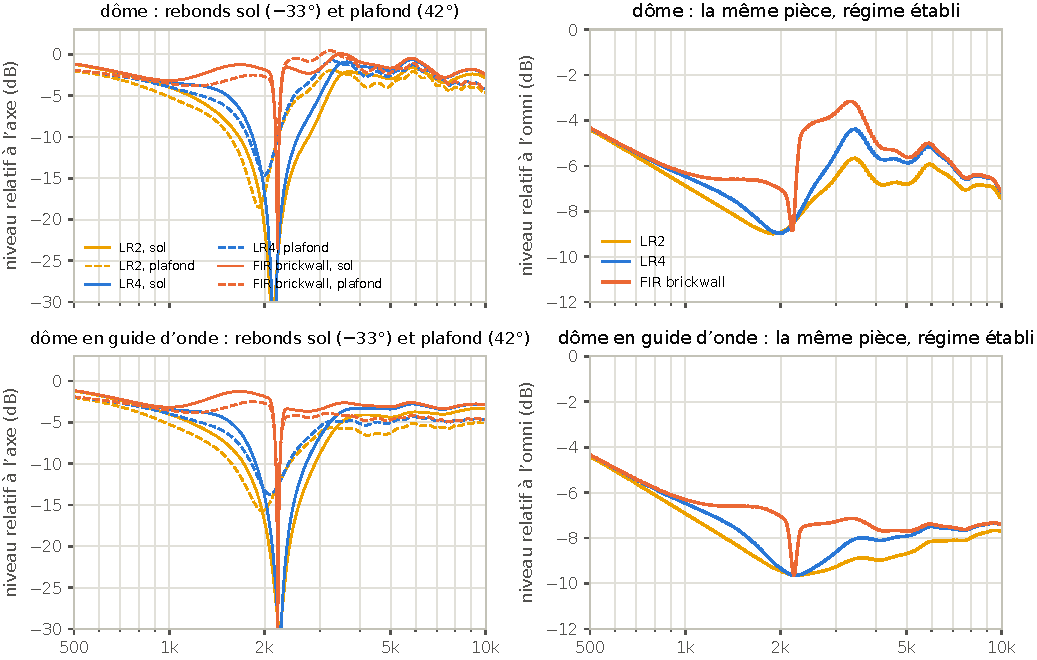
\includegraphics[width=\textwidth]{paths}
\caption{Le salon de la figure~\ref{fig:setup}. À gauche~: la réponse de l'enceinte dans les directions
des rebonds sur le sol et sur le plafond, relative à l'axe, avec trois filtres. À droite~: la réponse en
régime établi de la même pièce, relative à une source omnidirectionnelle.}
\label{fig:paths}
\end{figure}

Dans le salon de la figure~\ref{fig:setup}, le rebond sur le sol part à $-33^\circ$, près du premier zéro,
et celui sur le plafond à $+42^\circ$ (figure~\ref{fig:paths}). Avec le dôme nu et le LR4, le rebond sur
le sol présente un creux de \nnotchDomeLrFourFloorDepth\,dB, large de \nnotchDomeLrFourFloorWidth\,Hz à
$-6$\,dB de la droite (\nnotchDomeLrTwoFloorWidth\,Hz avec le LR2)~; celui du brickwall fait
\nnotchDomeFirFloorDepth\,dB de profondeur et \nnotchDomeFirFloorWidth\,Hz de large. Au plafond, plus loin
du zéro~: \nnotchDomeLrFourCeilingDepth\,dB sur \nnotchDomeLrFourCeilingWidth\,Hz avec le LR4,
\nnotchDomeFirCeilingDepth\,dB sur \nnotchDomeFirCeilingWidth\,Hz avec le brickwall. Avec le guide
d'onde, les creux sont aussi profonds, et ceux du brickwall aussi étroits. Dans la réponse moyennée de
la même pièce, le LR4 ne laisse qu'un creux de 2 à 3\,dB, large d'une octave environ.

\begin{figure}[t]
\centering
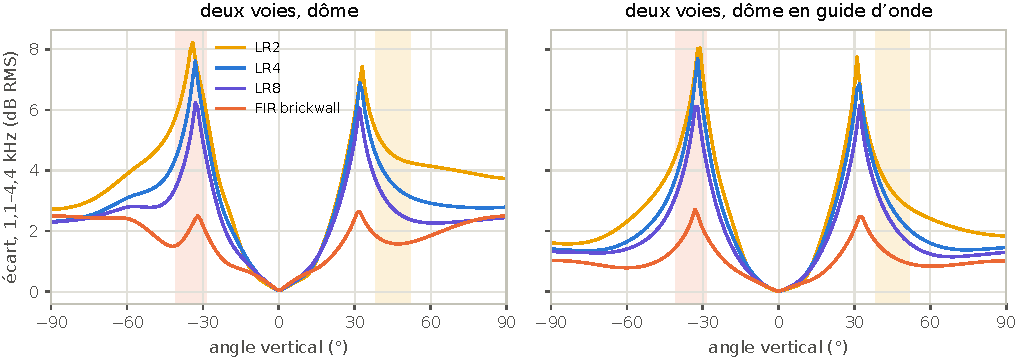
\includegraphics[width=\textwidth]{vertical_colouration}
\caption{Écart de la réponse dans chaque direction de l'orbite verticale, à moins d'une octave du
raccordement, et directions des rebonds sur le sol et le plafond des pièces (zones colorées, de 10 à
90\,\%).}
\label{fig:verticalcol}
\end{figure}

Le long de l'orbite verticale (figure~\ref{fig:verticalcol}), l'écart culmine près du premier zéro, à
$-33^\circ$ et $+32^\circ$ avec le dôme nu~: 8,3 et 7,4\,dB RMS avec le LR2, 7,6 et 7,0 avec le LR4, 6,5 et
6,1 avec le LR8, 2,5 et 2,7 avec le brickwall. Les rebonds sur le sol des 300 pièces se placent sur le
pic inférieur, ceux sur le plafond sur l'épaule du pic supérieur.

\subsection{Résultats}

\begin{table}[t]
\centering
\caption{Courbes moyennées, à moins d'une octave du raccordement (dB)~: écart RMS à la droite de la PIR,
de la PIR aux poids ajustés, du régime établi et du son précoce des pièces (médiane des 300)~; creux le
plus profond de la PIR et du régime établi des pièces.}
\label{tab:anomalies}
\small
\begin{tabular}{lrrrrrr}
\toprule
& \multicolumn{4}{c}{écart RMS} & \multicolumn{2}{c}{creux le plus profond} \\
& PIR & ajustée & pièces & pièces & PIR & pièces \\
& & & établi & précoce & & établi \\
\midrule
\rows{anomalies}
\bottomrule
\end{tabular}
\end{table}

\begin{table}[t]
\centering
\caption{Coloration des trajets, deux voies debout~: écart RMS à moins d'une octave du raccordement (dB),
pondéré par la PIR, par les poids ajustés et par les pièces (médiane des 300)~: tous les trajets, les
premières réflexions, les rebonds sur le sol et le plafond~; et creux le plus profond des rebonds sur le
sol et le plafond.}
\label{tab:colouration}
\small
\begin{tabular}{lrrrrrr}
\toprule
& poids & poids & pièces & pièces & pièces & sol, plafond \\
& PIR & ajustés & établi & réflexions & sol, plafond & creux max. \\
\midrule
\rows{colouration}
\bottomrule
\end{tabular}
\end{table}

\begin{figure}[t]
\centering
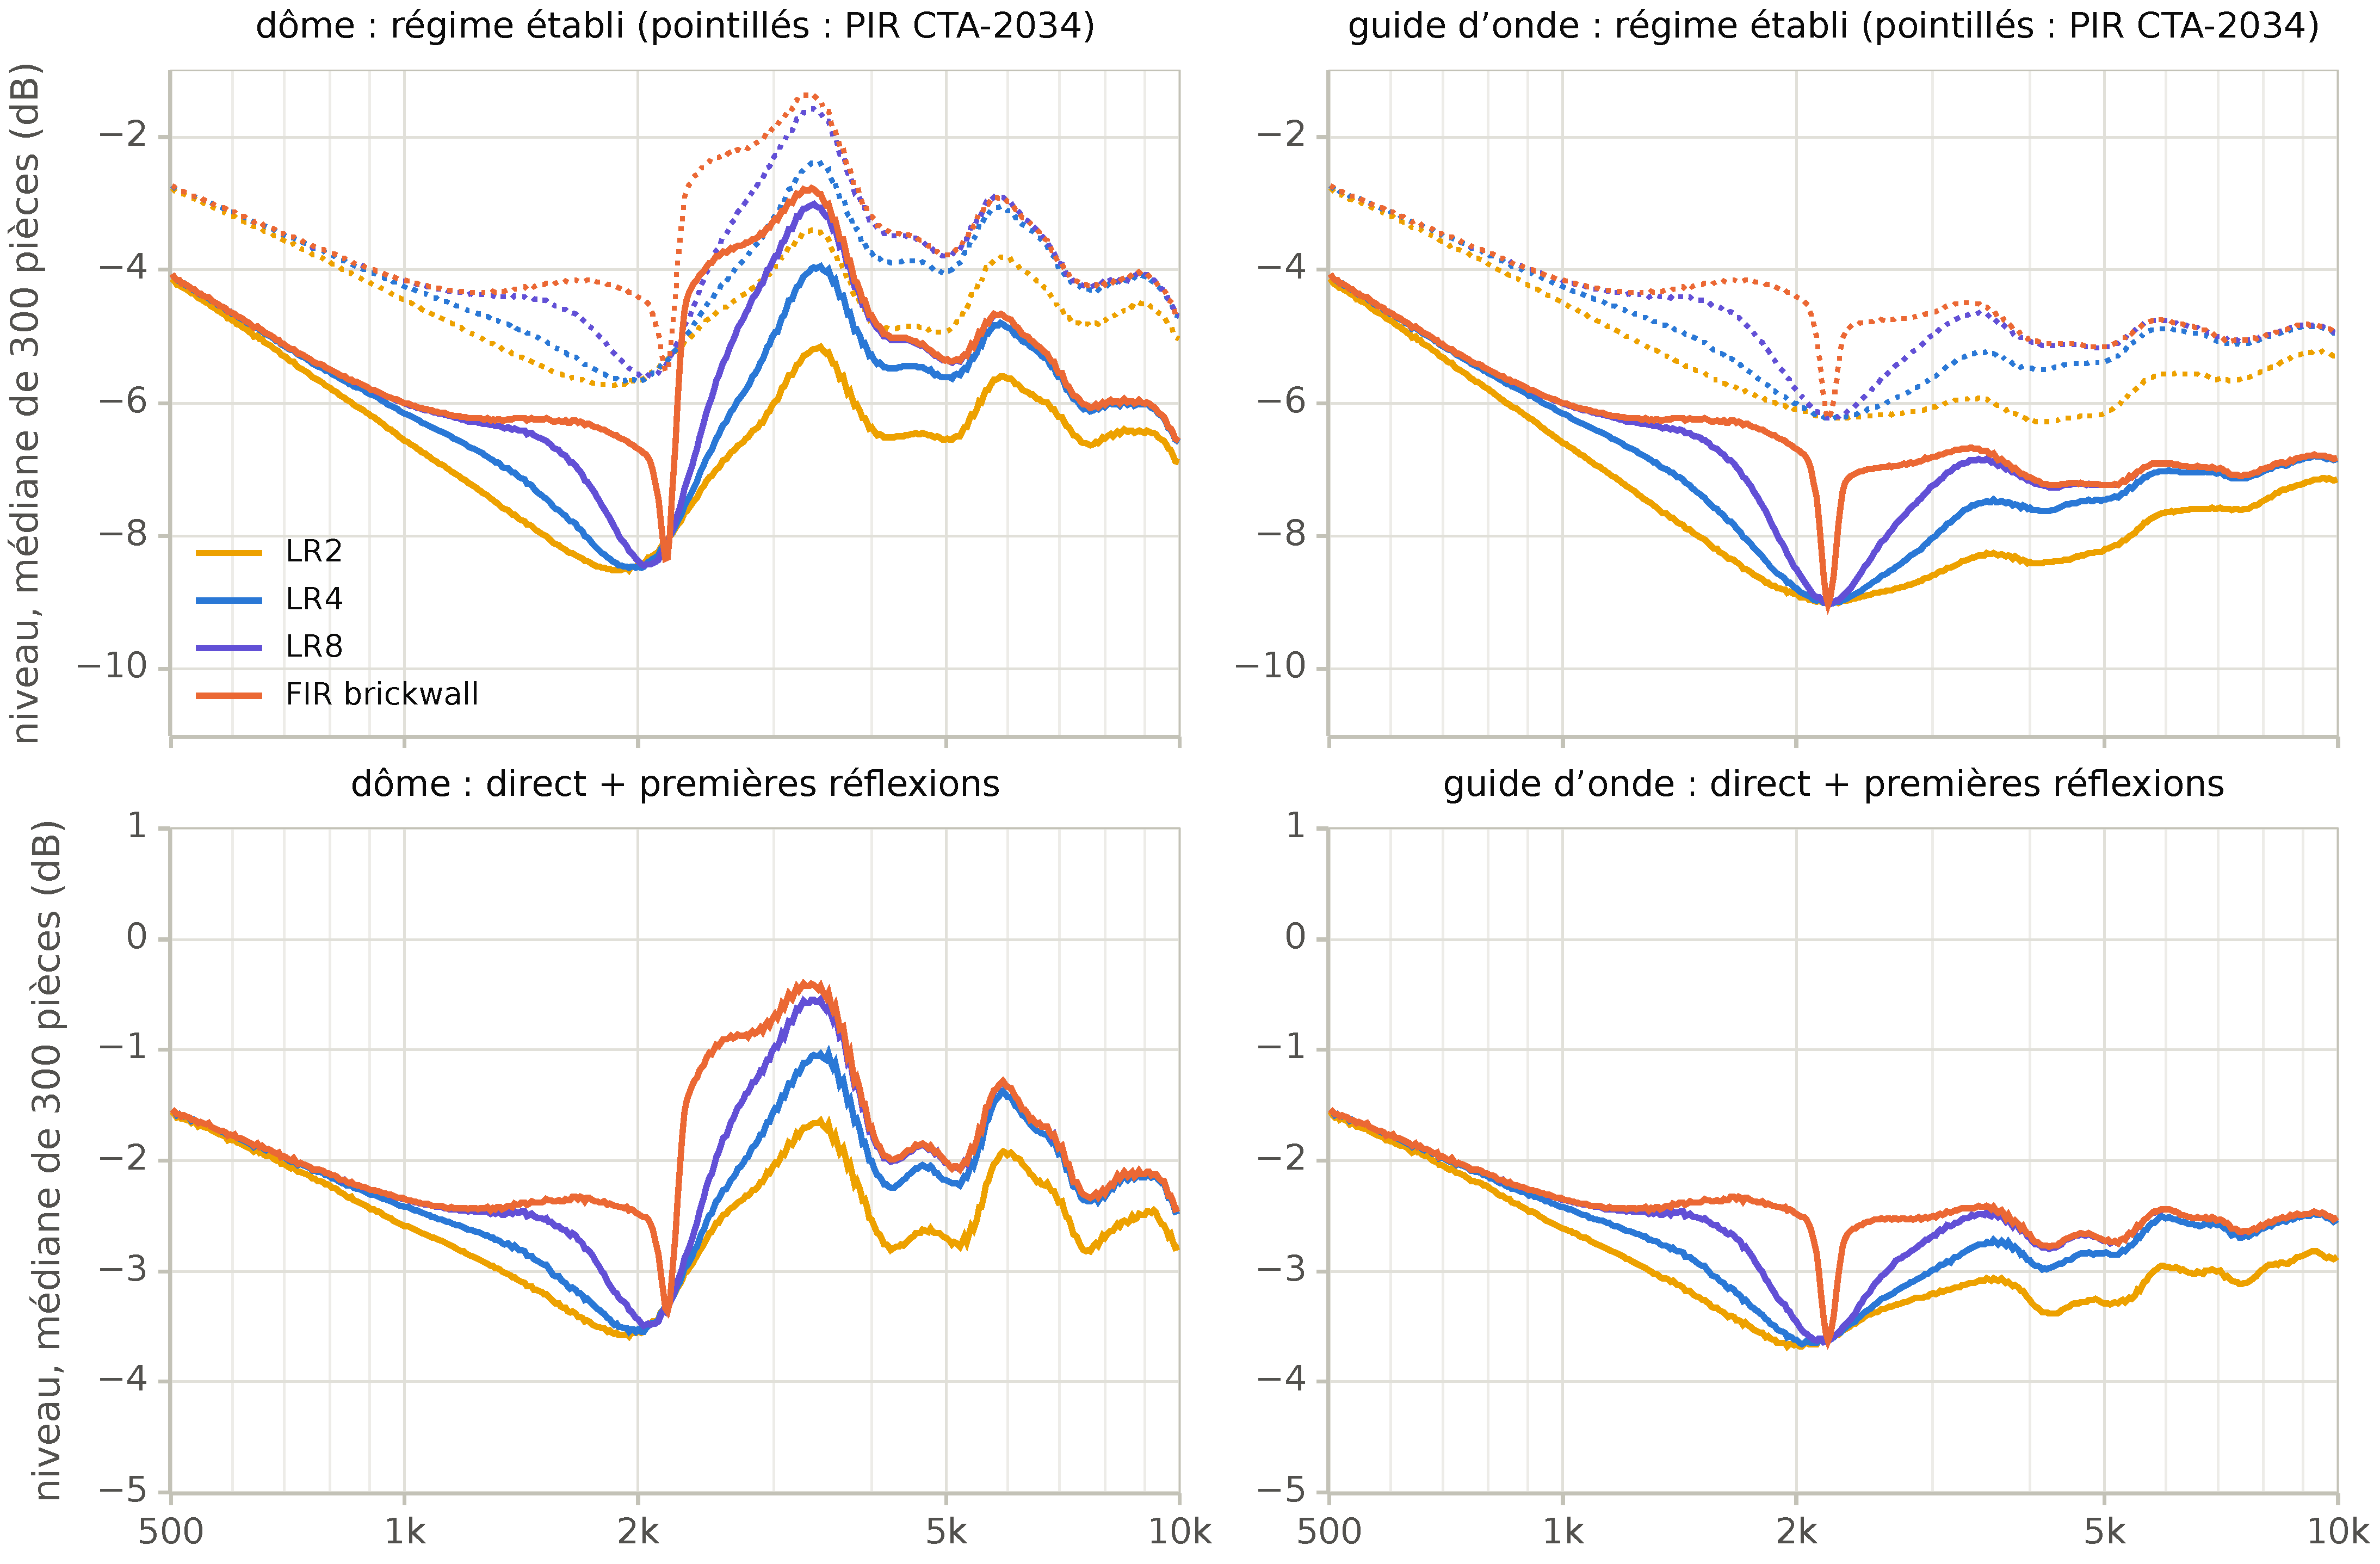
\includegraphics[width=\textwidth]{crossovers}
\caption{Réponse médiane des 300 pièces avec les quatre filtres, en régime établi (en haut, la PIR en
pointillés) et pour le son précoce (en bas)~; dôme nu (à gauche), dôme en guide d'onde (à droite).}
\label{fig:crossovers}
\end{figure}

\begin{figure}[t]
\centering
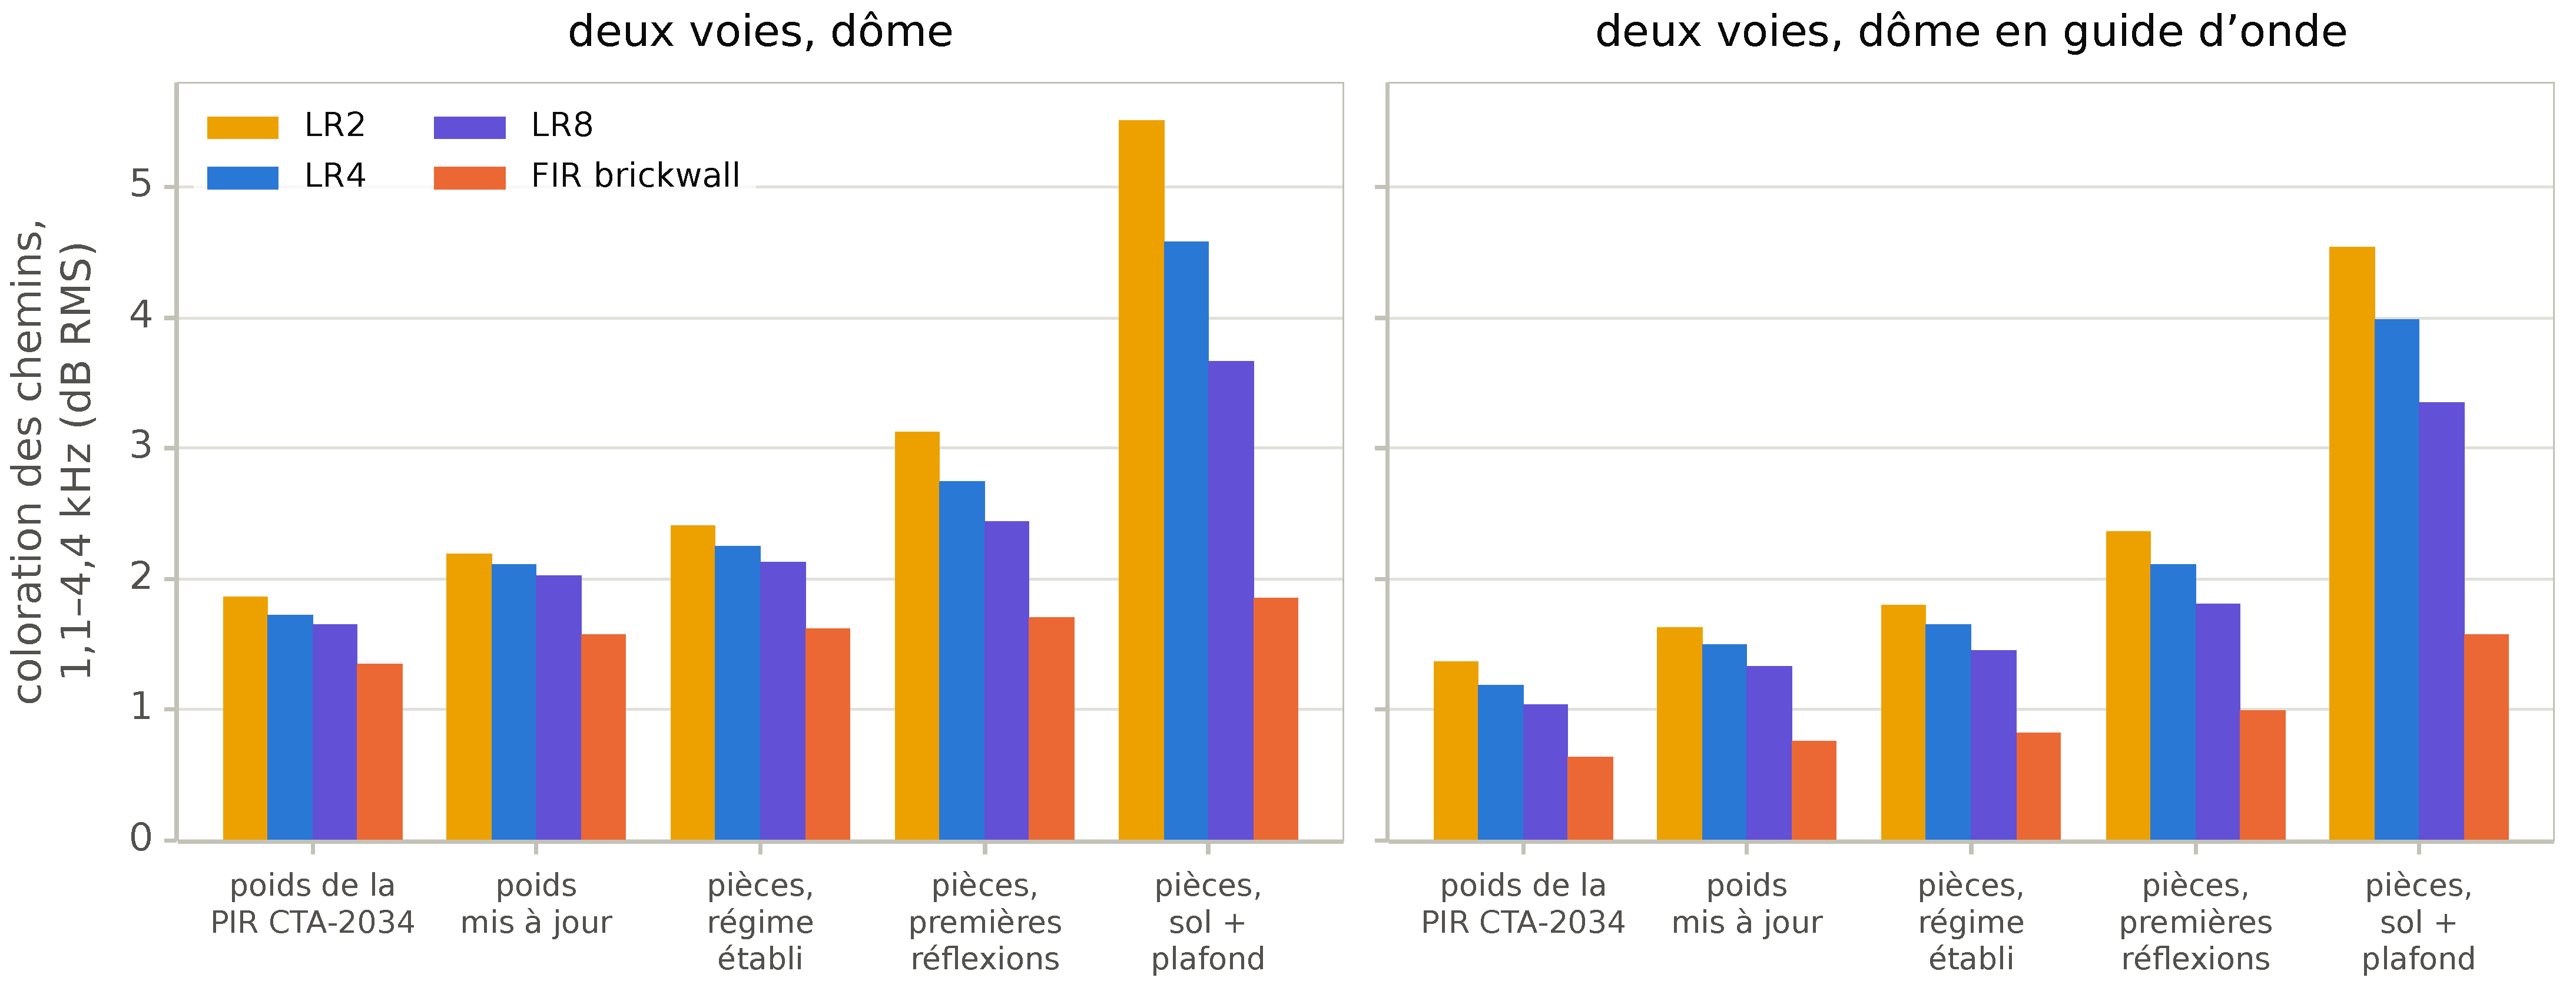
\includegraphics[width=\textwidth]{colouration}
\caption{Coloration des trajets avec les quatre filtres, deux voies debout.}
\label{fig:colouration}
\end{figure}

\emph{Les moyennes flattent le filtre à faible pente} (tableau~\ref{tab:anomalies},
figure~\ref{fig:crossovers}). À la fréquence de raccordement, les quatre filtres donnent la même réponse,
chaque haut-parleur à la moitié de l'amplitude et en phase~; ils diffèrent par la largeur de la bande où
les deux haut-parleurs jouent ensemble. Dans la réponse moyennée des pièces, le LR2 du dôme nu s'écarte
de la droite de \ncurveDomeLrTwoRoom\,dB RMS, le LR4 de \ncurveDomeLrFourRoom\ et le brickwall de
\ncurveDomeFirRoom~; les creux les plus profonds font \ncurveDomeLrTwoRoomDip, \ncurveDomeLrFourRoomDip\ et
\ncurveDomeFirRoomDip\,dB, celui du brickwall étant son creux étroit au raccordement. Avec le dôme nu, le
brickwall transforme en outre le large creux du LR4 en une marche d'environ 3\,dB vers le rayonnement
plus large du dôme, et la courbe moyennée n'en est pas plus régulière. Avec le guide d'onde, la marche
disparaît~: \ncurveWgLrFourRoom\ contre \ncurveWgFirRoom\,dB (\ncurveWgLrTwoRoom\ avec le LR2). La PIR
classe les filtres dans le même ordre.

\emph{Les trajets les classent dans l'ordre inverse} (tableau~\ref{tab:colouration},
figure~\ref{fig:colouration}). Les rebonds sur le sol et le plafond portent \ncolDomeLrTwoVert\,dB RMS avec
le LR2, \ncolDomeLrFourVert\ avec le LR4 et \ncolDomeFirVert\ avec le brickwall (dôme nu~;
\ncolWgLrTwoVert, \ncolWgLrFourVert\ et \ncolWgFirVert\ avec le guide d'onde)~: du LR4 au brickwall,
\ncolDomeRedVert\ et \ncolWgRedVert\,\% de moins, et le LR2 fait \ncolDomeLrTwoMoreVert\,\% de plus que le
LR4. Sur l'ensemble des premières réflexions, le brickwall en retire \ncolDomeRedRefl\ et
\ncolWgRedRefl\,\%, sur tous les trajets en régime établi \ncolDomeRedSteady\ et \ncolWgRedSteady\,\%. Le
creux le plus profond des rebonds sur le sol et le plafond change peu (\ncolDomeLrFourVertDip\ contre
\ncolDomeFirVertDip\,dB avec le dôme nu, \ncolWgLrFourVertDip\ contre \ncolWgFirVertDip\,dB avec le guide
d'onde)~: les creux du brickwall sont aussi profonds, mais dix à treize fois plus étroits, environ un
trentième d'octave contre un tiers.

\emph{Ce que les moyennes cachent.} Avec le dôme nu et le LR4, les rebonds sur le sol et le plafond
portent \ncolDomeLrFourVert\,dB RMS à moins d'une octave du raccordement, et la réponse moyennée des
pièces en montre \ncurveDomeLrFourRoom~: la moyenne divise la coloration par 3,4 environ. Avec le LR2,
elle la divise par 5 (\ncolDomeLrTwoVert\ contre \ncurveDomeLrTwoRoom\,dB), avec le brickwall par 1,4. Plus
la pente est faible, plus la bande où les haut-parleurs interfèrent est large, plus nombreuses sont les
directions qui voient le creux à des fréquences différentes, et plus la moyenne le comble.

\emph{Les poids de la norme} accordent à la coloration des trajets moins d'importance que les pièces
(\ncolDomeLrFourPir\ contre \ncolDomeLrFourSteady\,dB avec le dôme nu et le LR4), parce que la PIR
s'appuie sur la fenêtre d'écoute, où les lobes verticaux ne se voient pas~; ils montrent un gain un peu
plus faible du brickwall (\ncolDomeRedPir\ contre \ncolDomeRedSteady\,\% avec le dôme nu, \ncolWgRedPir\
contre \ncolWgRedSteady\,\% avec le guide d'onde). Les poids mis à jour se situent entre les deux.

\clearpage
\subsection{Interférences aux oreilles}
\label{sec:interference}

Jusqu'ici, toutes les réponses somment les trajets en puissance, comme si chacun s'entendait seul. En un
point fixe, le son direct et les réflexions s'ajoutent en pression~: une réflexion retardée de $\tau$
creuse la réponse tous les $1/\tau$, en peigne. Pour voir ce que ce peigne change à la comparaison, le
son direct et les images jusqu'au troisième ordre ont été sommés avec leurs phases en quatorze
points~: les deux oreilles, distantes de 17,5\,cm et sans tête, de sept positions de la tête (la
position de référence, 10\,cm de part et d'autre, 10\,cm en avant et en arrière, 5\,cm plus haut et plus
bas). Chaque image garde la racine de son poids énergétique comme coefficient de réflexion réel et
positif, et la réponse de l'enceinte dans la direction où part son trajet~; le champ diffus reste sommé
en énergie. L'oreille ne résout pas le peigne serré d'une réflexion tardive~: chaque réponse est donc
lissée par les filtres auditifs de Glasberg et Moore \cite{glasberg1990}, des exponentielles arrondies
larges d'une ERB (\nerbCrossover\,Hz au raccordement, environ un sixième d'octave), calculées sur une grille
de 4\,Hz, avant que l'on prenne son écart à moins d'une octave du raccordement. L'énergie des images
coïncide avec celle de l'étude à $\ncohCheck$\,dB près. Une source omnidirectionnelle dans les mêmes pièces
montre les peignes que les pièces produisent seules.

\begin{table}[t]
\centering
\caption{Écart à moins d'une octave du raccordement (dB RMS, médiane des 300 pièces) des trajets sommés
en énergie au point de référence, puis avec leurs phases~: en un point (médiane des quatorze), aux deux
oreilles moyennées en puissance, sur les quatorze points moyennés. Deux voies debout~; réponses lissées
par les filtres auditifs.}
\label{tab:coherent}
\small
\begin{tabular}{lrrrrrrrr}
\toprule
& \multicolumn{4}{c}{régime établi} & \multicolumn{4}{c}{son précoce} \\
\cmidrule(lr){2-5}\cmidrule(lr){6-9}
& énergie & point & oreilles & 14 pts & énergie & point & oreilles & 14 pts \\
\midrule
\rows{coherent}
\bottomrule
\end{tabular}
\end{table}

\begin{figure}[t]
\centering
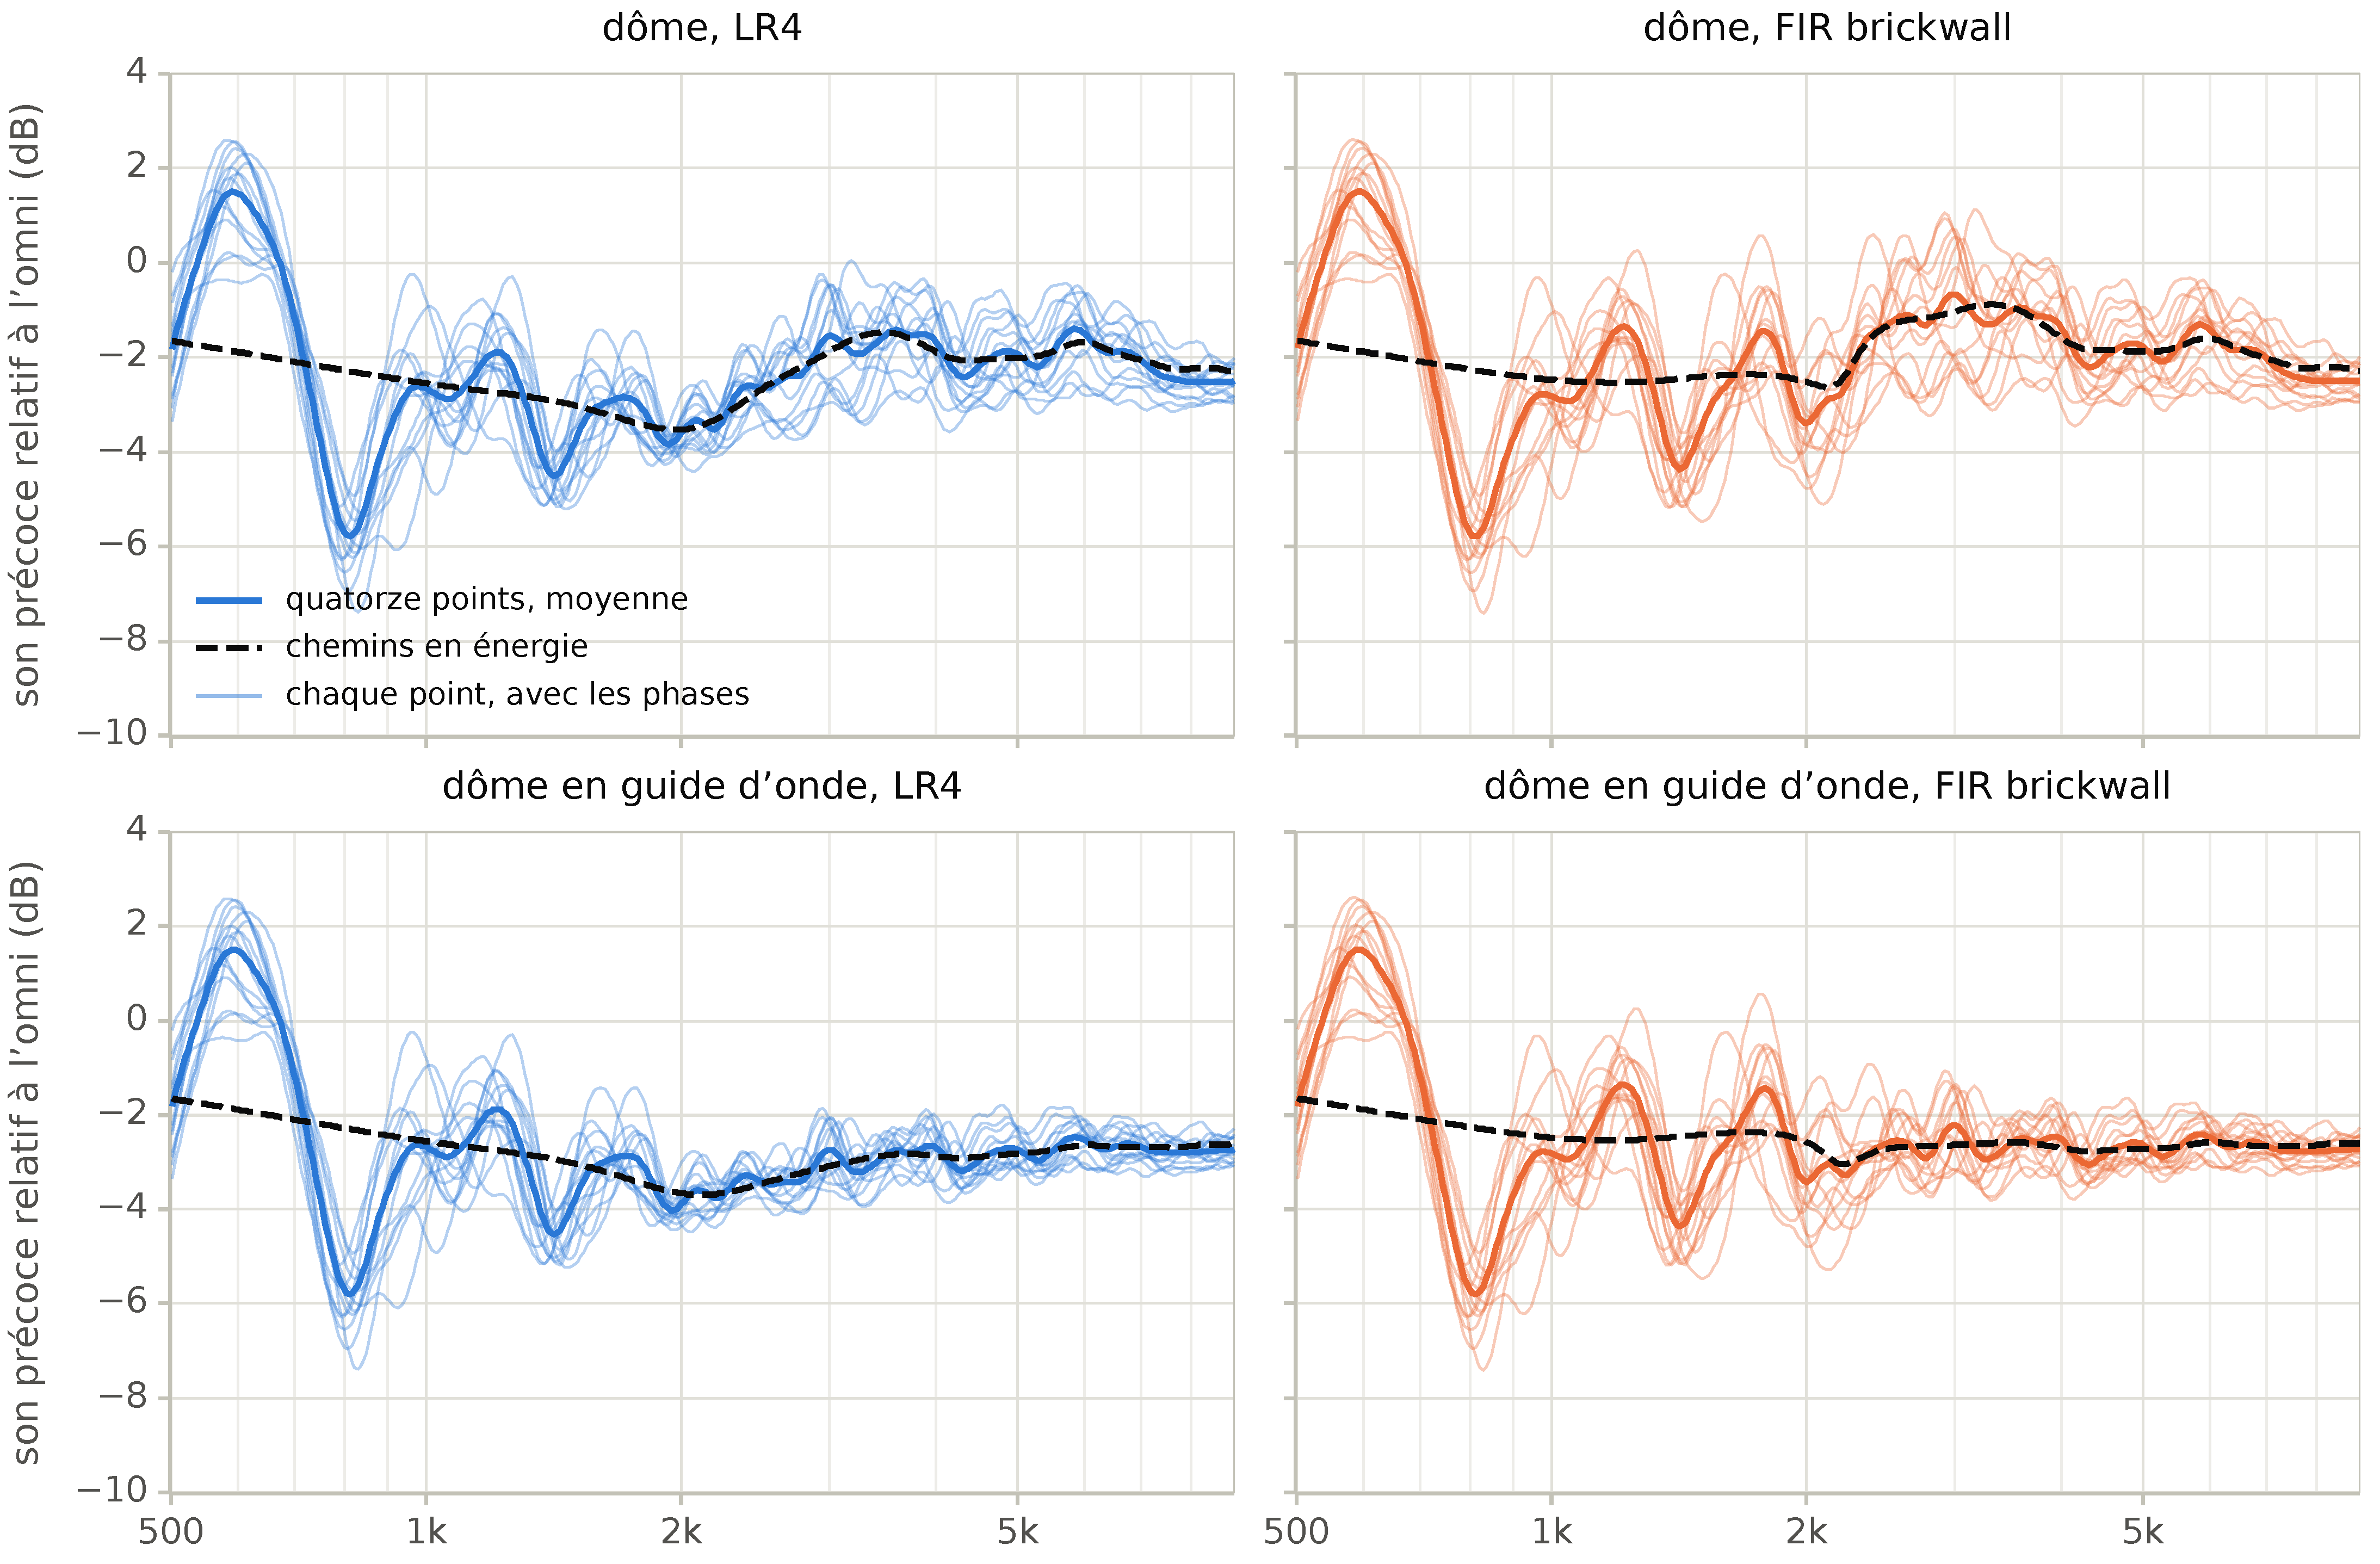
\includegraphics[width=\textwidth]{interference}
\caption{Son précoce dans le salon de la figure~\ref{fig:setup}, relatif à une source
omnidirectionnelle~: les trajets sommés en énergie au point de référence (tirets), et avec leurs phases
en chacun des quatorze points (traits fins) et en moyenne sur ces points (trait épais)~; lissage par les
filtres auditifs.}
\label{fig:interference}
\end{figure}

\begin{figure}[t]
\centering
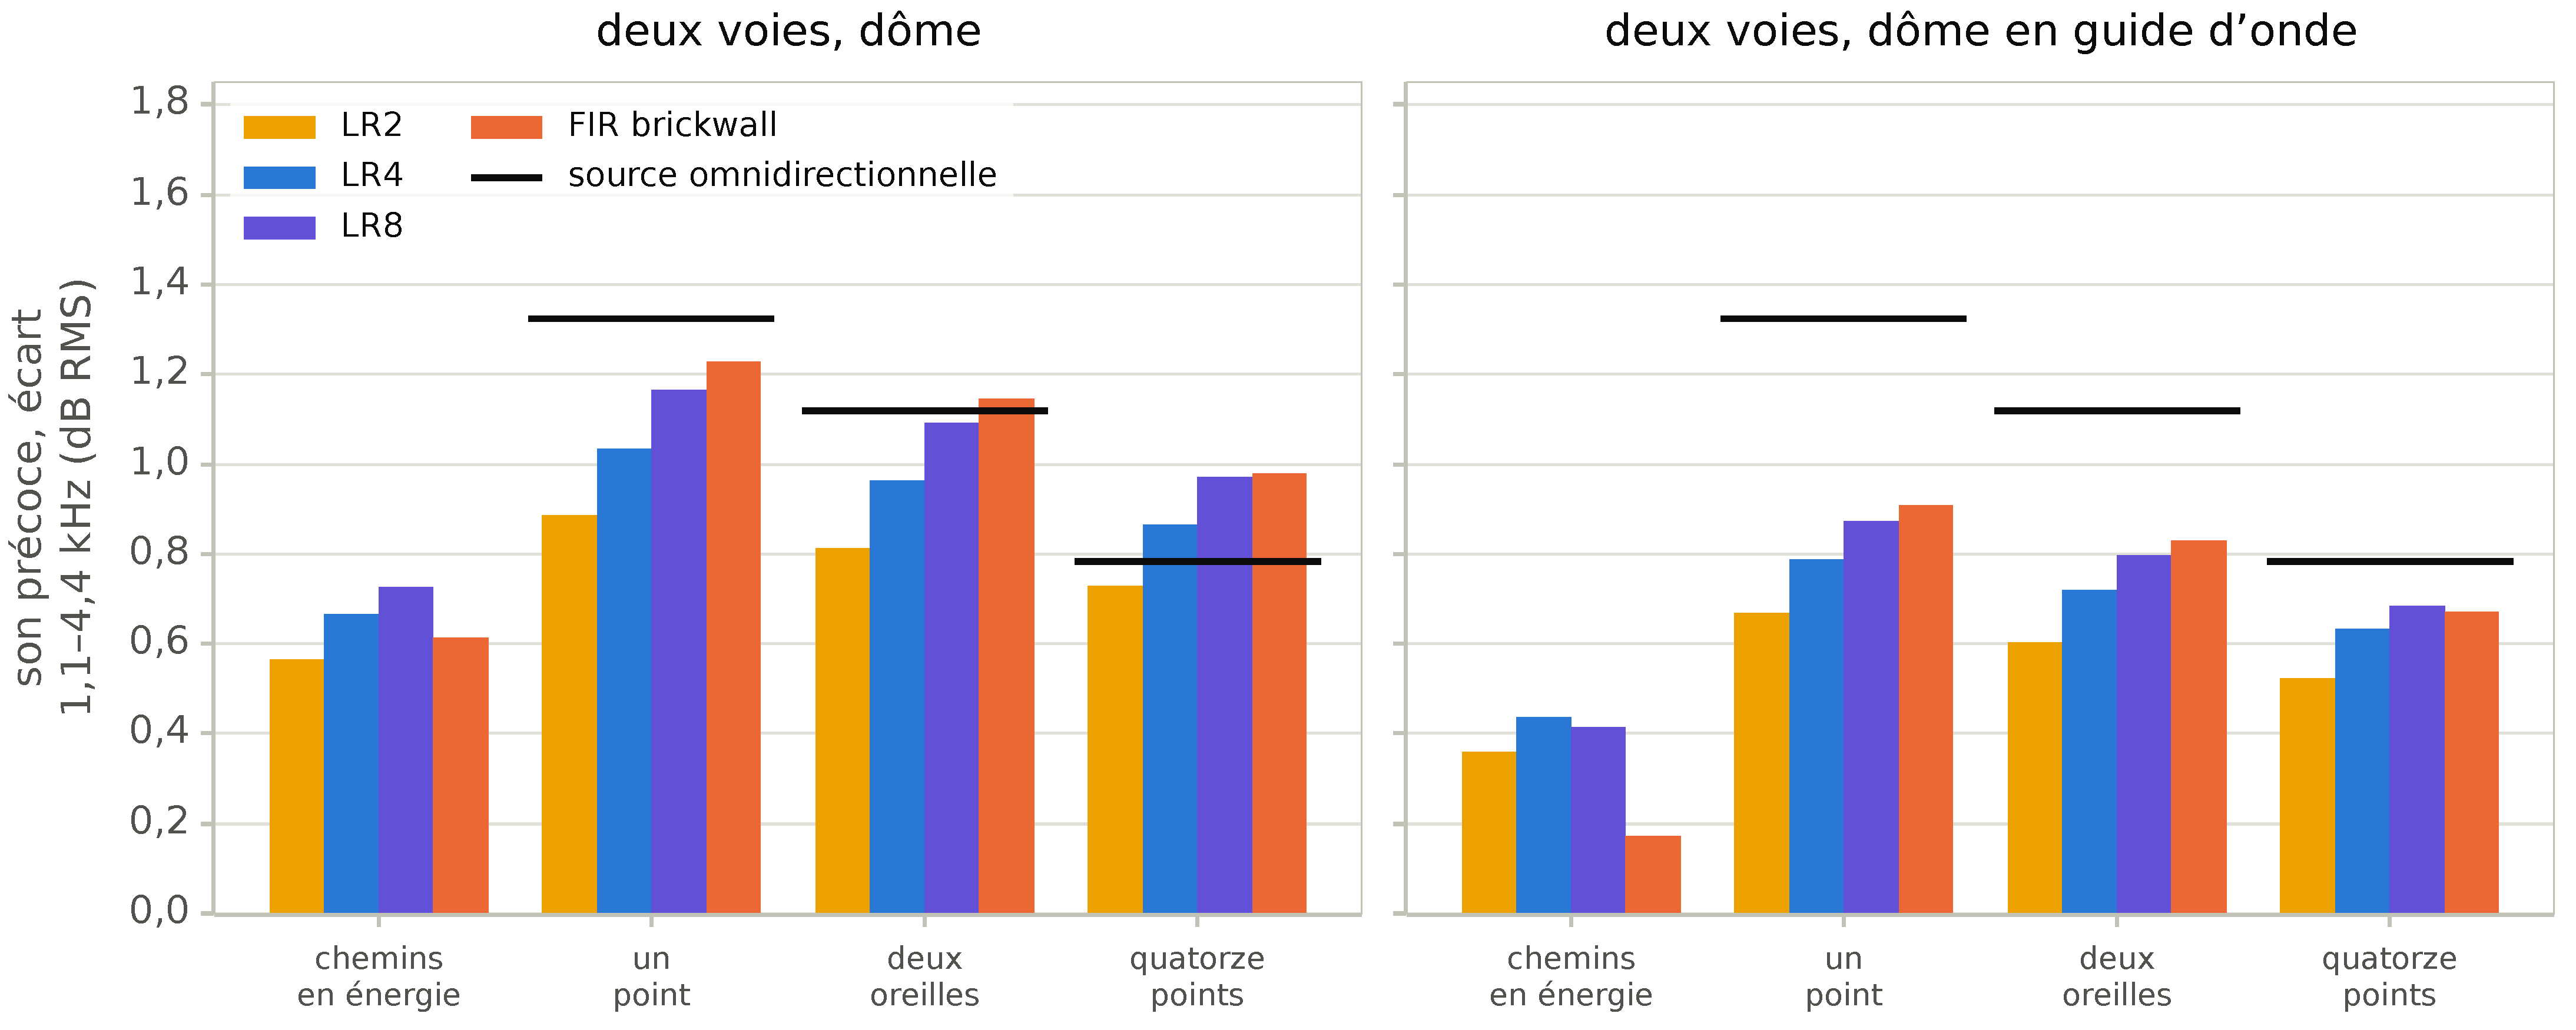
\includegraphics[width=\textwidth]{interference_summary}
\caption{Écart du son précoce à moins d'une octave du raccordement (médiane des 300 pièces)~: les trajets
sommés en énergie, puis avec leurs phases en un point, aux deux oreilles moyennées, sur les quatorze
points moyennés. Traits noirs~: une source omnidirectionnelle, les peignes des seules pièces.}
\label{fig:interference-summary}
\end{figure}

\emph{En régime établi, les phases changent peu de chose} (tableau~\ref{tab:coherent}). Le champ diffus,
sommé en énergie, comble les peignes~: en un point, l'écart augmente de \ncohSteadyGainMin\ à
\ncohSteadyGainMax\,dB, et les filtres gardent leur ordre (dôme nu~: LR2 \ncohDomeLrTwoSteadyPoint, LR4
\ncohDomeLrFourSteadyPoint, brickwall \ncohDomeFirSteadyPoint\,dB~; guide d'onde~: \ncohWgLrFourSteadyPoint\
avec le LR4 contre \ncohWgFirSteadyPoint\ avec le brickwall). Les peignes de la source omnidirectionnelle
laissent \ncohOmniSteadyPoint\,dB.

\emph{Le son précoce en un point est une autre affaire} (figures~\ref{fig:interference}
et~\ref{fig:interference-summary}). Le son direct y rencontre les rebonds sur le sol et le plafond,
\ndelayFloor\ et \ndelayCeiling\,ms plus tard dans la pièce médiane~: leurs peignes, espacés de quelques
centaines de hertz, ont à peu près la largeur des filtres auditifs et résistent au lissage. La source
omnidirectionnelle montre \ncohOmniEarlyPoint\,dB RMS à moins d'une octave du raccordement en un point,
plus qu'aucun filtre en énergie (\ncohDomeLrEightEarlyEnergy\,dB au plus, le LR8 avec le dôme nu). Les
enceintes se placent entre les deux, de \ncohDomeLrTwoEarlyPoint\ (LR2) à \ncohDomeFirEarlyPoint\,dB
(brickwall) avec le dôme nu, de \ncohWgLrTwoEarlyPoint\ à \ncohWgFirEarlyPoint\,dB avec le guide d'onde, et le
brickwall passe au dernier rang~: le plus régulier en énergie avec le guide d'onde
(\ncohWgFirEarlyEnergy\ contre \ncohWgLrFourEarlyEnergy\,dB pour le LR4), il est le plus irrégulier en un
point. Le creux du Linkwitz-Riley retire les rebonds sur le sol et le plafond autour du raccordement, et
leur peigne avec eux~: dans le salon, les quatorze points rejoignent la somme en énergie vers 2\,kHz avec
le LR4, pas avec le brickwall, qui laisse intacts les réflexions et leur peigne. Moyenner les deux
oreilles ou les quatorze points réduit les écarts sans les combler (\ncohWgLrFourEarlySpatial\ contre
\ncohWgFirEarlySpatial\,dB sur les quatorze points avec le guide d'onde).

Ce que mesure le peigne, c'est la pièce, pas le filtre~: une source sans filtre le montre partout, et un
filtre qui creuse les réflexions près de sa fréquence l'y retire, avec une partie de leur énergie.
Dire si cela s'entend mieux revient aux tests d'écoute. Le peigne d'une réflexion isolée colore moins
le son pour deux oreilles que pour une seule (décoloration binaurale \cite{salomons1995}), et le spectre
propre des réflexions, que mesure la coloration des trajets, est ce que l'oreille attribue à la pièce.
Les interférences laissent donc intact le tableau du régime établi~; en un point fixe, elles échangent la
coloration des réflexions par le filtre contre le peigne que ces réflexions provoquent.

% =============================================================================================
\section{Discussion}

\subsection{Les trois objections}

\emph{Le poids de la verticale.} Dans ces pièces, le sol et le plafond fournissent aux premières
réflexions une part d'énergie aussi grande que celle que leur donnent les premières réflexions de la
norme, et leurs rebonds partent là où la norme regarde. Ils arrivent bien les premiers, et quand les
murs latéraux sont traités ils en fournissent la moitié, un peu plus que les 40\,\% de la norme.
L'objection vaut en revanche pour la puissance~: les deux orbites pèsent autant le plan sans
interférence que celui qui en a, et manquent la moitié de la puissance perdue par les lobes. Ce biais
est le même pour les lobes horizontaux et verticaux~; pour une enceinte debout, il tombe sur les
verticaux.

\emph{La fenêtre d'écoute.} Ce n'est pas son étroitesse verticale qui cache les lobes~: le son direct d'un
auditeur assis ne voit pas davantage les lobes verticaux, et l'enceinte couchée montre ce dont la
fenêtre protège. Ce qui les cache, c'est la moyenne que partagent toutes les courbes, celle de la pièce
comprise. Les rebonds sur le sol et le plafond d'une deux voies en LR4 portent des creux de 10 à 40\,dB,
larges d'un tiers d'octave, qui tombent à des fréquences différentes selon la direction~; les moyennes
les réduisent à un creux de 2\,dB. Plus la pente est faible, plus les moyennes flattent le filtre~: la
courbe dans la pièce et la PIR désignent le LR2 comme le plus régulier des Linkwitz-Riley, alors que ses
réflexions sont les plus colorées. Sous cette forme, l'objection tient.

\emph{Le filtre brickwall.} Il réduit d'environ 60\,\% la coloration des rebonds sur le sol et le
plafond, avec ou sans guide d'onde, et de 38 à 53\,\% celle de l'ensemble des premières réflexions. Ses
creux sont aussi profonds que ceux des Linkwitz-Riley, et dix à treize fois plus étroits. Que la courbe
dans la pièce devienne plus régulière dépend des haut-parleurs~: quand le boomer devient directif au
raccordement et que le tweeter ne l'est pas, le brickwall transforme le creux des lobes en une marche de
directivité. Raccorder les directivités (un guide d'onde) et resserrer la bande où les deux
haut-parleurs jouent ensemble (un filtre raide) traitent deux causes différentes de la coloration hors
axe.

\subsection{Une pondération mise à jour}

Ce que demandent les pièces se formule simplement~:
\begin{itemize}
\item la puissance sur la sphère, que donnent aujourd'hui les scanners en champ proche et les mesures
sphériques, plutôt que sur deux orbites~;
\item pour la réponse dans la pièce en régime établi, environ $0,1\,\mathrm{LW} + 0,9\,\mathrm{SP}$~: la
pièce intègre surtout la puissance acoustique, le son direct ajoutant un peu de poids vers l'avant~;
\item pour le son précoce, qui porte les réflexions entendues avec le son direct, environ
$0,4\,\mathrm{LW} + 0,5\,\mathrm{ER} + 0,1\,\mathrm{SP}$.
\end{itemize}
Ajusté sur l'énergie reçue, le premier jeu de poids prédit les pièces à leur propre dispersion près. Il
ne défait pas la moyenne pour autant~: aucune moyenne pondérée de réponses en puissance ne montre le
creux que porte une réflexion isolée. Celui-ci se lit direction par direction, sur les cartes polaires
ou avec une mesure comme la coloration des trajets utilisée ici, dans les directions où partent les
rebonds sur le sol et le plafond, de $-30$ à $-40^\circ$ et de $+40$ à $+50^\circ$ aux distances d'écoute
habituelles.

\subsection{Limites}

Les pièces sont des boîtes rectangulaires, d'absorption uniforme par paroi en dehors des zones
traitées, avec des coefficients de manuel et un modèle hybride spéculaire et diffus~; les vraies pièces
ont des meubles sur les trajets, des ouvertures, des formes irrégulières. Leur réverbération et leurs
parts d'énergie découlent de la constante de salle et ne sont pas propres à ce modèle, mais la part de
chaque première réflexion dépend des matériaux au point de réflexion. Les trajets sont sommés en
énergie, sauf à la section~\ref{sec:interference}, où les images se rencontrent avec leurs phases en des
points sans tête~; les modes de la pièce sous 200\,Hz environ sortent du cadre de l'étude. Le son précoce est lui aussi une somme d'énergie~; l'audition pèse les réflexions
autrement que par leur énergie (décoloration binaurale des réflexions latérales, poids du rebond sur le
sol dans le plan médian \cite{bech1996,olive1989}), ce qu'aucune pondération de réponses en puissance ne
saisit. Les mesures de coloration sont physiques~: un creux étroit s'entend moins qu'un creux large de
même profondeur \cite{bucklein1981}, et l'écart RMS n'en tient compte qu'à travers sa largeur.
L'enceinte est une seule deux voies bibliothèque, en deux versions~; une trois voies, une cardioïde, une
colonne ou une distance d'écoute plus grande changeraient les chiffres, pas la méthode. Enfin, l'étude
part de la CTA-2034-A~; sa révision B n'a pas été vérifiée.

% =============================================================================================
\section{Conclusion}

Vues comme des pondérations des directions de la sphère, les courbes de la CTA-2034 et une pièce se
comparent directement. Dans 300 pièces domestiques simulées, la norme cherche les premières réflexions
dans les bonnes directions et donne au sol et au plafond la bonne part de leur énergie~; sa fenêtre
d'écoute correspond à la place des auditeurs. Ses poids, eux, ne correspondent pas à l'énergie reçue~:
les premières réflexions portent \nfirstShare\,\% de l'énergie en régime établi, et non 44\,\%, et les
pièces sont prédites à leur propre dispersion près par environ $0,1\,\mathrm{LW} + 0,9\,\mathrm{SP}$ avec la
puissance de toute la sphère, que deux orbites sous-estiment là où les haut-parleurs interfèrent. Toute
moyenne, celle de la pièce comprise, comble les creux que le filtre dessine dans chaque réflexion, et
flatte d'abord les filtres à faible pente. Lu trajet par trajet, un filtre brickwall retire environ
60\,\% de la coloration des rebonds sur le sol et le plafond~; il ne donne une réponse plus régulière dans
la pièce que si les directivités des haut-parleurs se raccordent. Sommés avec leurs phases aux
oreilles, les trajets laissent le régime établi tel quel~; en un point fixe, le son précoce porte le
peigne des rebonds sur le sol et le plafond, qu'un creux de Linkwitz-Riley retire près du raccordement
avec les réflexions, et qu'une écoute à deux oreilles atténue.

% =============================================================================================
\begin{thebibliography}{99}

\bibitem{cta2034a} ANSI/CTA-2034-A, \emph{Standard Method of Measurement for In-Home Loudspeakers},
Consumer Technology Association, 2015 (R2020).

\bibitem{cta2034b} ANSI/CTA-2034-B, \emph{Standard Method of Measurement for In-Home Loudspeakers},
Consumer Technology Association, juillet 2024.

\bibitem{devantier2002} A. Devantier, \og Characterizing the Amplitude Response of Loudspeaker
Systems\fg{}, 113\ieme{} convention de l'AES, preprint 5638, 2002.

\bibitem{toole2018} F. E. Toole, \emph{Sound Reproduction: The Acoustics and Psychoacoustics of
Loudspeakers and Rooms}, 3\ieme{} éd., Routledge, 2018.

\bibitem{olive2004} S. E. Olive, \og A Multiple Regression Model for Predicting Loudspeaker Preference
Using Objective Measurements: Part II -- Development of the Model\fg{}, 117\ieme{} convention de l'AES,
preprint 6190, 2004.

\bibitem{demion2026} A. Demion, \og Brickwall FIR Crossovers Against LR24 on Four-Way Studio
Monitors\fg{}, blog DEM Audio, octobre 2026, \url{https://demaudio.com/blog/brickwall-fir-vs-lr24/}.

\bibitem{turntable2026} \og Polar Measurements on a Small Turntable: How Well Can the Rotation Center Be
Corrected?\fg{}, rapport technique, 2026,
\url{https://github.com/Arnwald/turntable-rotation-center-study}.

\bibitem{urban2004} M. Urban, C. Heil, C. Pignon, C. Combet, P. Bauman, \og The Distributed Edge Dipole
(DED) Model for Cabinet Diffraction Effects\fg{}, \emph{J. Audio Eng. Soc.}, vol.~52, n\textsuperscript{o}~10,
2004.

\bibitem{allen1979} J. B. Allen, D. A. Berkley, \og Image Method for Efficiently Simulating Small-Room
Acoustics\fg{}, \emph{J. Acoust. Soc. Am.}, vol.~65, n\textsuperscript{o}~4, p.~943--950, 1979.

\bibitem{kuttruff2016} H. Kuttruff, \emph{Room Acoustics}, 6\ieme{} éd., CRC Press, 2016.

\bibitem{hopkins1948} H. F. Hopkins, N. R. Stryker, \og A Proposed Loudness-Efficiency Rating for
Loudspeakers and the Determination of System Power Requirements for Enclosures\fg{}, \emph{Proc. IRE},
vol.~36, n\textsuperscript{o}~3, p.~315--335, 1948.

\bibitem{iso9613} ISO 9613-1, \emph{Acoustique -- Atténuation du son lors de sa propagation à l'air
libre -- Partie 1~: Calcul de l'absorption atmosphérique}, 1993.

\bibitem{diaz2005} C. D\'iaz, A. Pedrero, \og The reverberation time of furnished rooms in
dwellings\fg{}, \emph{Applied Acoustics}, vol.~66, n\textsuperscript{o}~8, 2005.

\bibitem{bech1996} S. Bech, \og Timbral aspects of reproduced sound in small rooms. II\fg{}, \emph{J.
Acoust. Soc. Am.}, vol.~99, n\textsuperscript{o}~6, 1996.

\bibitem{olive1989} S. E. Olive, F. E. Toole, \og The Detection of Reflections in Typical Rooms\fg{},
\emph{J. Audio Eng. Soc.}, vol.~37, n\textsuperscript{o}~7/8, 1989.

\bibitem{bucklein1981} R. Bücklein, \og The Audibility of Frequency Response Irregularities\fg{}, \emph{J.
Audio Eng. Soc.}, vol.~29, n\textsuperscript{o}~3, p.~126--131, 1981.

\bibitem{glasberg1990} B. R. Glasberg, B. C. J. Moore, \og Derivation of auditory filter shapes from
notched-noise data\fg{}, \emph{Hearing Research}, vol.~47, p.~103--138, 1990.

\bibitem{salomons1995} A. M. Salomons, \emph{Coloration and Binaural Decoloration of Sound due to
Reflections}, thèse de doctorat, Delft University of Technology, 1995.

\end{thebibliography}

\end{document}
